%%%%%%%%%%%%%%%%%%%%%%%%%%%%%%%%%%%%%%%%%
% Uppsala University Assignment Title Page 
% LaTeX Template
% Version 1.0 (27/12/12)
%
% This template has been downloaded from:
% http://www.LaTeXTemplates.com
%
% Original author:
% WikiBooks (http://en.wikibooks.org/wiki/LaTeX/Title_Creation)
% Modified by Elsa Slattegard to fit Uppsala university
% License:
% CC BY-NC-SA 3.0 (http://creativecommons.org/licenses/by-nc-sa/3.0/)

%\title{Title page with logo}
%----------------------------------------------------------------------------------------
%	PACKAGES AND OTHER DOCUMENT CONFIGURATIONS
%----------------------------------------------------------------------------------------

\documentclass[12pt]{article}

\usepackage{tikz,lipsum,lmodern}
\usepackage[most]{tcolorbox}

\usepackage[utf8]{inputenc}
\usepackage[greek,english]{babel}
\usepackage{alphabeta}
\usepackage{amsmath}
\usepackage{gfsartemisia}
\usepackage{graphicx}

\usepackage{float}
\usepackage[colorinlistoftodos]{todonotes}
\usepackage{tabularx}
\usepackage[myheadings]{fullpage}
\usepackage{enumitem}
\PassOptionsToPackage{hyphens}{url}\usepackage{hyperref}
\usepackage{tikz}
\usepackage[nottoc]{tocbibind} %Adds "References" to the table of contents
\usepackage{xcolor} % to access the named colour LightGray
\definecolor{LightGray}{gray}{0.9}

\usepackage{caption}
\usepackage{subcaption}

\usepackage[edges]{forest}
\definecolor{folderbg}{RGB}{124,166,198}
\definecolor{folderborder}{RGB}{110,144,169}

%================ file tree =====================%
\usepackage[edges]{forest}
\definecolor{folderbg}{RGB}{124,166,198}
\definecolor{folderborder}{RGB}{110,144,169}
\newlength\Size
\setlength\Size{4pt}
\tikzset{%
	folder/.pic={%
		\filldraw [draw=folderborder, top color=folderbg!50, bottom color=folderbg] (-1.05*\Size,0.2\Size+5pt) rectangle ++(.75*\Size,-0.2\Size-5pt);
		\filldraw [draw=folderborder, top color=folderbg!50, bottom color=folderbg] (-1.15*\Size,-\Size) rectangle (1.15*\Size,\Size);
	},
	file/.pic={%
		\filldraw [draw=folderborder, top color=folderbg!5, bottom color=folderbg!10] (-\Size,.4*\Size+5pt) coordinate (a) |- (\Size,-1.2*\Size) coordinate (b) -- ++(0,1.6*\Size) coordinate (c) -- ++(-5pt,5pt) coordinate (d) -- cycle (d) |- (c) ;
	},
}
\forestset{%
	declare autowrapped toks={pic me}{},
	pic dir tree/.style={%
		for tree={%
			folder,
			font=\ttfamily,
			grow'=0,
		},
		before typesetting nodes={%
			for tree={%
				edge label+/.option={pic me},
			},
		},
	},
	pic me set/.code n args=2{%
		\forestset{%
			#1/.style={%
				inner xsep=2\Size,
				pic me={pic {#2}},
			}
		}
	},
	pic me set={directory}{folder},
	pic me set={file}{file},
}

%=================================================%


\usepackage{tabto}
\usepackage{minted}


\hyphenpenalty=10000


\usepackage{geometry}
\geometry{
	a4paper,
	total={170mm,257mm},
	left=20mm,
	top=20mm,
}


\addto\captionsenglish{% Replace "english" with the language you use
	\renewcommand{\contentsname}%
	{Περιεχόμενα}%
}

\addto\captionsenglish{
	\renewcommand{\partname}{}
}
\renewcommand{\thepart}{}

\makeatletter
\renewcommand{\fnum@figure}{Εικόνα \thefigure}
\makeatother


\renewcommand{\H}{\textlozenge}

%=====fonts==========%
%\usepackage{libertine}


%====================%





%=============header + footer ======================%
%

\usepackage{fancyhdr}

\pagestyle{fancy}
\fancyhf{}
\rhead{Σύγχρονα θέματα Τεχνολογίας Λογισμικού 
\includegraphics[width=0.7cm]{UNIPI_(logo).png}}
\lhead{Πανεπιστήμιο Πειραιώς \\ Τμήμα Πληροφορικής}
\cfoot{Σελίδα \thepage}

% 

%\setlength\headheight{47pt}
%=====================================================%



%\setcounter{secnumdepth}{0} % sections are level 1

\begin{document}
	
	\begin{titlepage}
		
		\newcommand{\HRule}{\rule{\linewidth}{0.5mm}} % Defines a new command for the horizontal lines, change thickness here
		
		\center % Center everything on the page
		
		%----------------------------------------------------------------------------------------
		%	HEADING SECTIONS
		%----------------------------------------------------------------------------------------
		
		\textsc{\LARGE Πανεπιστήμιο Πειραιώς}\\[1.5cm] % Name of your university/college
		
\includegraphics[scale=0.6]{UNIPI_(logo).png}\\[1cm] % Include a department/university logo - this will require the graphicx package
		\textsc{\Large Τμήμα Πληροφορικής}\\[0.5cm] % Major heading such as course name
		\textsc{\large Σύγχρονα θέματα Τεχνολογίας Λογισμικού - Λογισμικό για κινητές συσκευές}\\[0.5cm] % Minor heading such as course title
		
		%----------------------------------------------------------------------------------------
		%	TITLE SECTION
		%----------------------------------------------------------------------------------------
		
		\HRule \\[0.4cm]
		{ \Large \bfseries University Application}\\[0.4cm] % Title of your document
		{ \Large \bfseries Εγχειρίδιο χρήσης}\\[0.4cm] % Title of your document
		\HRule \\[1.5cm]
		
		%----------------------------------------------------------------------------------------
		%	AUTHOR SECTION
		%----------------------------------------------------------------------------------------
		%
		
		% If you don't want a supervisor, uncomment the two lines below and remove the section above
		%\Large \emph{Author:}\\
		%John \textsc{Smith}\\[3cm] % Your name
		
		%----------------------------------------------------------------------------------------
		%	DATE SECTION
		%----------------------------------------------------------------------------------------
		
		
		
		\vfill % Fill the rest of the page with whitespace
		
	\end{titlepage}
	
	%\selectlanguage{greek}
	\tableofcontents
	%\selectlanguage{english}
	
	\newpage
	
	\section{Εισαγωγή}
	
	Το παρόν έγγραφο αποτελεί το εγχειρίδιο χρήσης για την εφαρμογή "UniveristyApp". Οι χρήστες απαιτείται να έχουν έναν λογαριασμό (username και password) προκειμένου να χρησιμοποιήσουν την εφαρμογή αυτή. Πιο συγκεκριμένα υπάρχουν 3 τύποι χρηστών: Φοιτητές, Καθηγητές και Διαχειριστές/Γραμματεία. Αφού οι χρήστες συνδεθούν (log in) με τους κωδικούς τους, θα έχουν πρόσβαση σε όλες τις λειτουργίες που τους αντιστοιχούν σύμφωνα με τύπου του λογαριασμού τους.
	
	\section{Η ιστοσελίδα}
	
	\subsection{Nav Bar}
	
	Στο πάνω μέρος της σελίδας υπάρχει μια μπάρα περιήγησης (navbar) η οποία περιέχει κάθε στιγμή όλους τους βασικούς συνδέσμους της ιστοσελίδας και είναι οι παρακάτω:
	
	\begin{figure}[H]
		\centering
		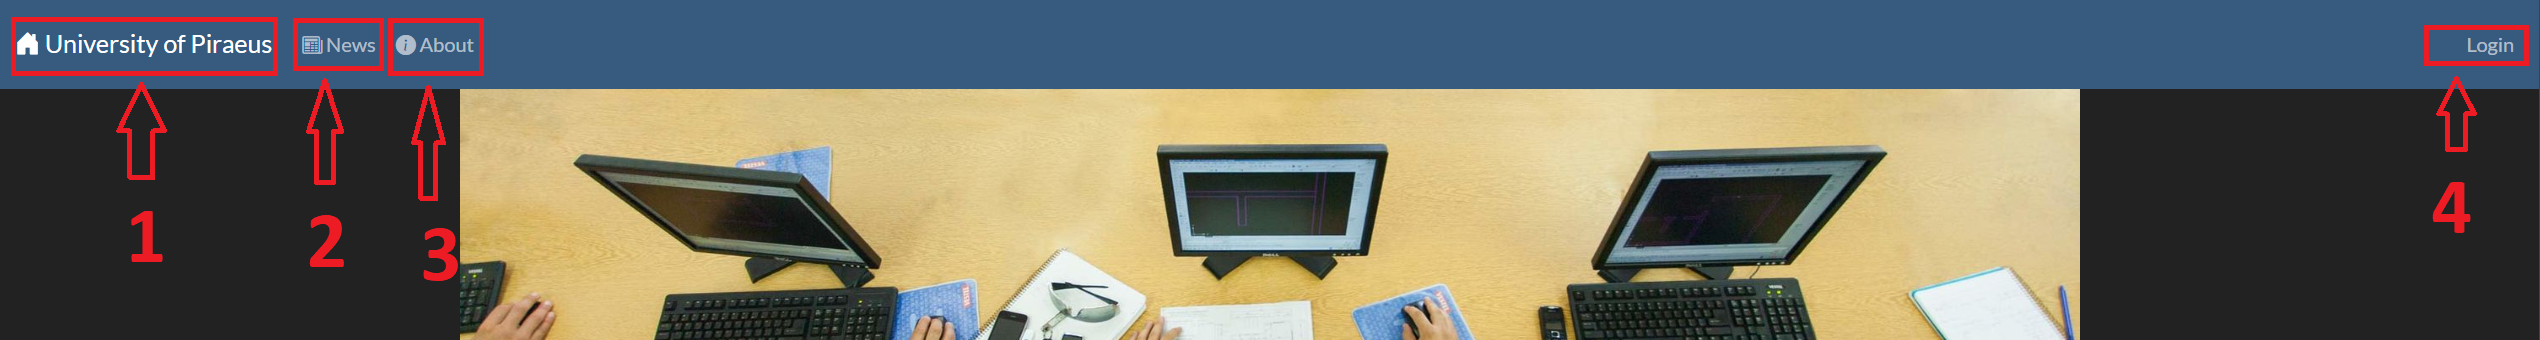
\includegraphics[width=0.95\textwidth]{homes2.png}
		\caption{Nav Bar}
		\label{fig:bar}
	\end{figure}
	
	\begin{enumerate}
		\item σύνδεσμος για το Home page 
		\item σύνδεσμος για το News page
		\item σύνδεσμος για το About page
		\item σύνδεσμος για το Log in page
	\end{enumerate}
	
	Όλες οι αναφερόμενες σελίδες θα εξηγηθούν σε επόμενες ενότητες. Επιπλέον ο σύνδεσμος 4 (Log in) θα αντικατασταθεί με το μενού επιλογών του χρήστη, εφόσον αυτός συνδεθεί επιτυχώς. Το μενού επιλογών έχει την παρακάτω μορφή.
	
	\begin{figure}[H]
		\centering
		\begin{subfigure}{.22\textwidth}
			\centering
			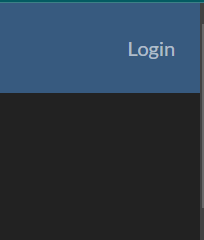
\includegraphics[width=.75\linewidth]{b0.png}
			\caption{Navbar χωρίς συνδεδεμένο χρήστη}
			\label{fig:sub21}
		\end{subfigure}%
		\begin{subfigure}{.22\textwidth}
			\centering
			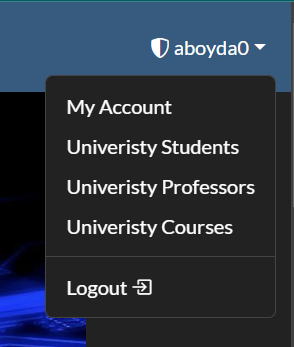
\includegraphics[width=.8\linewidth]{b1.png}
			\caption{Μενού επιλογών του Γραμματέα}
			\label{fig:sub22}
		\end{subfigure}
		\begin{subfigure}{.22\textwidth}
			\centering
			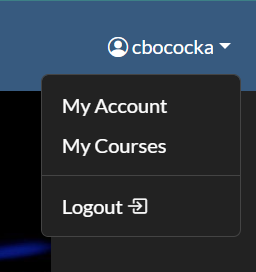
\includegraphics[width=.8\linewidth]{b2.png}
			\caption{Μενού επιλογών του Καθηγητή}
			\label{fig:sub23}
		\end{subfigure}
		\begin{subfigure}{.22\textwidth}
			\centering
			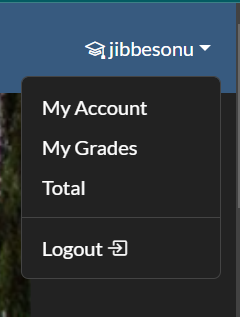
\includegraphics[width=.8\linewidth]{b3.png}
			\caption{Μενού επιλογών του Φοιτητή}
			\label{fig:sub24}
		\end{subfigure}
		\caption{}
		\label{fig:test1}
	\end{figure}
	
	Η πρώτη επιλογή είναι ίδια για όλους τους χρήστης και μεταβαίνει τον κάθε χρήστη στη σελίδα καλωσόρισής του. Στη συνέχεια ακολουθούν επιλογές που αφορούν τον συγκεκριμένο τύπο χρήστη που έκανε log in και τέλος υπάρχει η επιλογή log out.
	
	
	\subsection{Home page}
	
	Η κεντρική σελίδα (index) της εφαρμογής είναι η Home page. Σε αυτήν εμφανίζονται σύντομες και γενικές πληροφορίες για το Πανεπιστήμιο για το οποίο φτιάχτηκες η εφαρμογή. Στη συγκεκριμένη περίπτωση θεωρείται ότι το πανεπιστήμιο είναι το Πανεπιστήμιο Πειραιά. 
	
	\begin{figure}[H]
		\centering
		
\includegraphics[width=0.85\textwidth]{homes3.png}
		\caption{Home page}
		\label{fig:homes}
	\end{figure}
	
	
	Πατώντας στον σύνδεσμο 2 από το Nav bar (εικόνα \ref{fig:bar}) ο χρήστης μεταβαίνει στην ιστοσελίδα που περιέχει τα νέα του πανεπιστημίου.
	
	\begin{figure}[H]
		\centering
		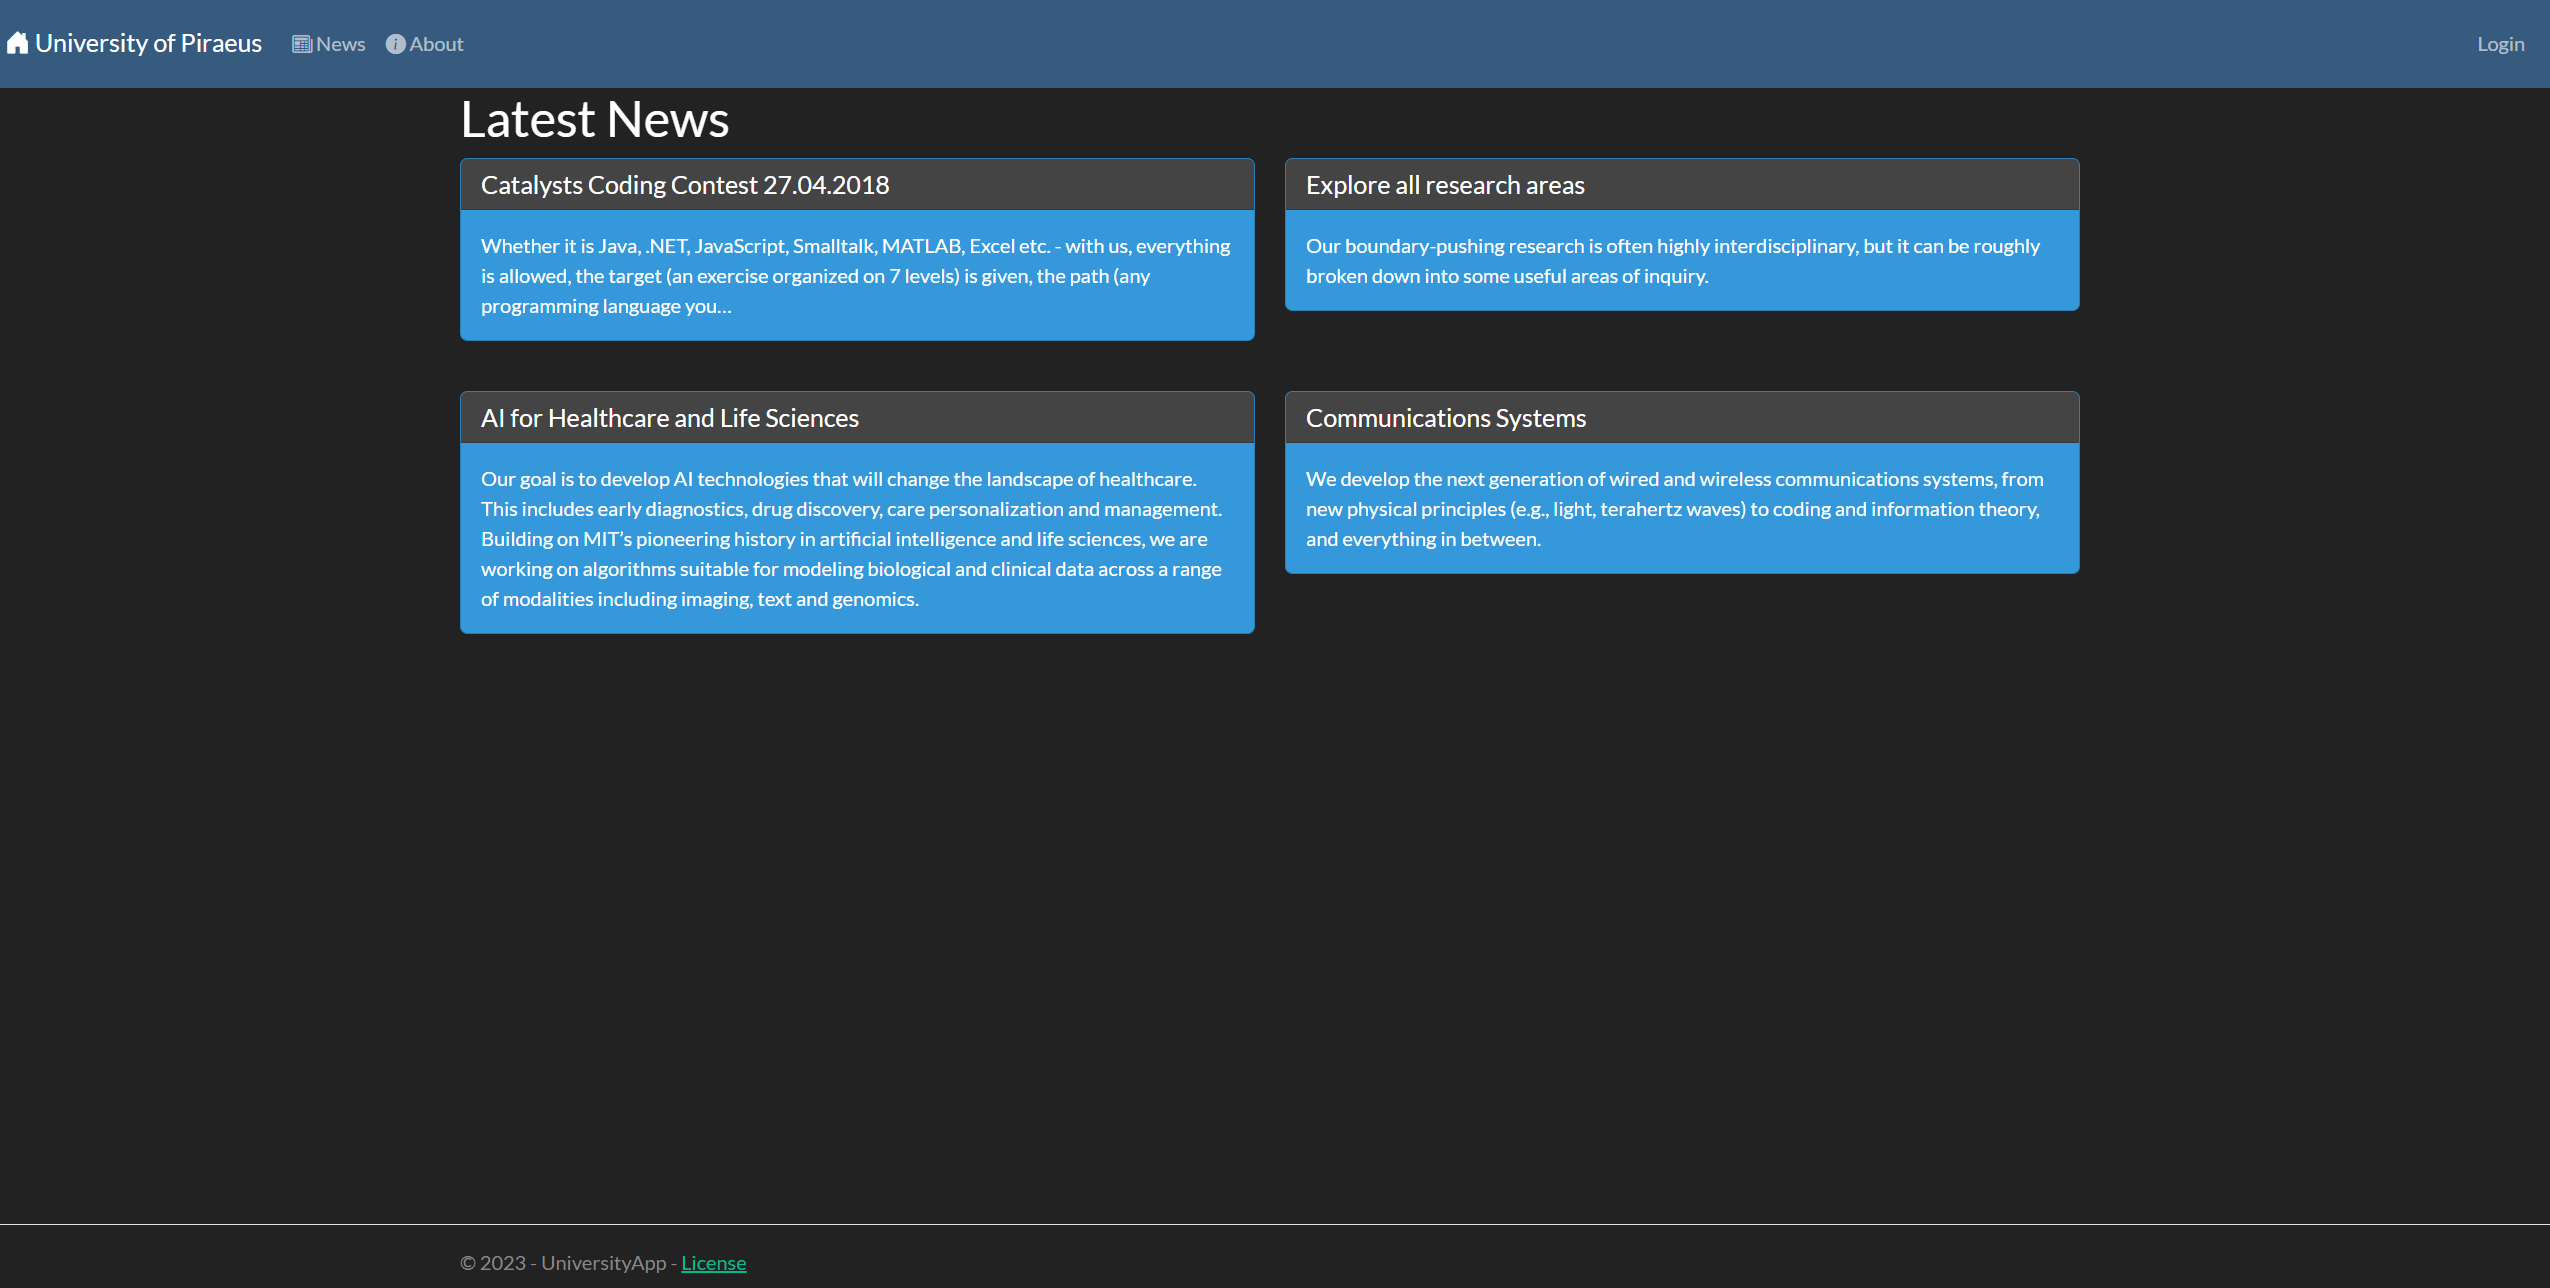
\includegraphics[width=0.85\textwidth]{news.png}
		\caption{News page}
		\label{fig:emptyView}
	\end{figure}
	
	Πατώντας στον σύνδεσμο 3 από το Nav bar (εικόνα \ref{fig:bar}) ο χρήστης μεταβαίνει σε μία ιστοσελίδα όπου περιέχονται τα ονόματα των δημιουργών της εφαρμογής.
	
	
	\begin{figure}[H]
		\centering
		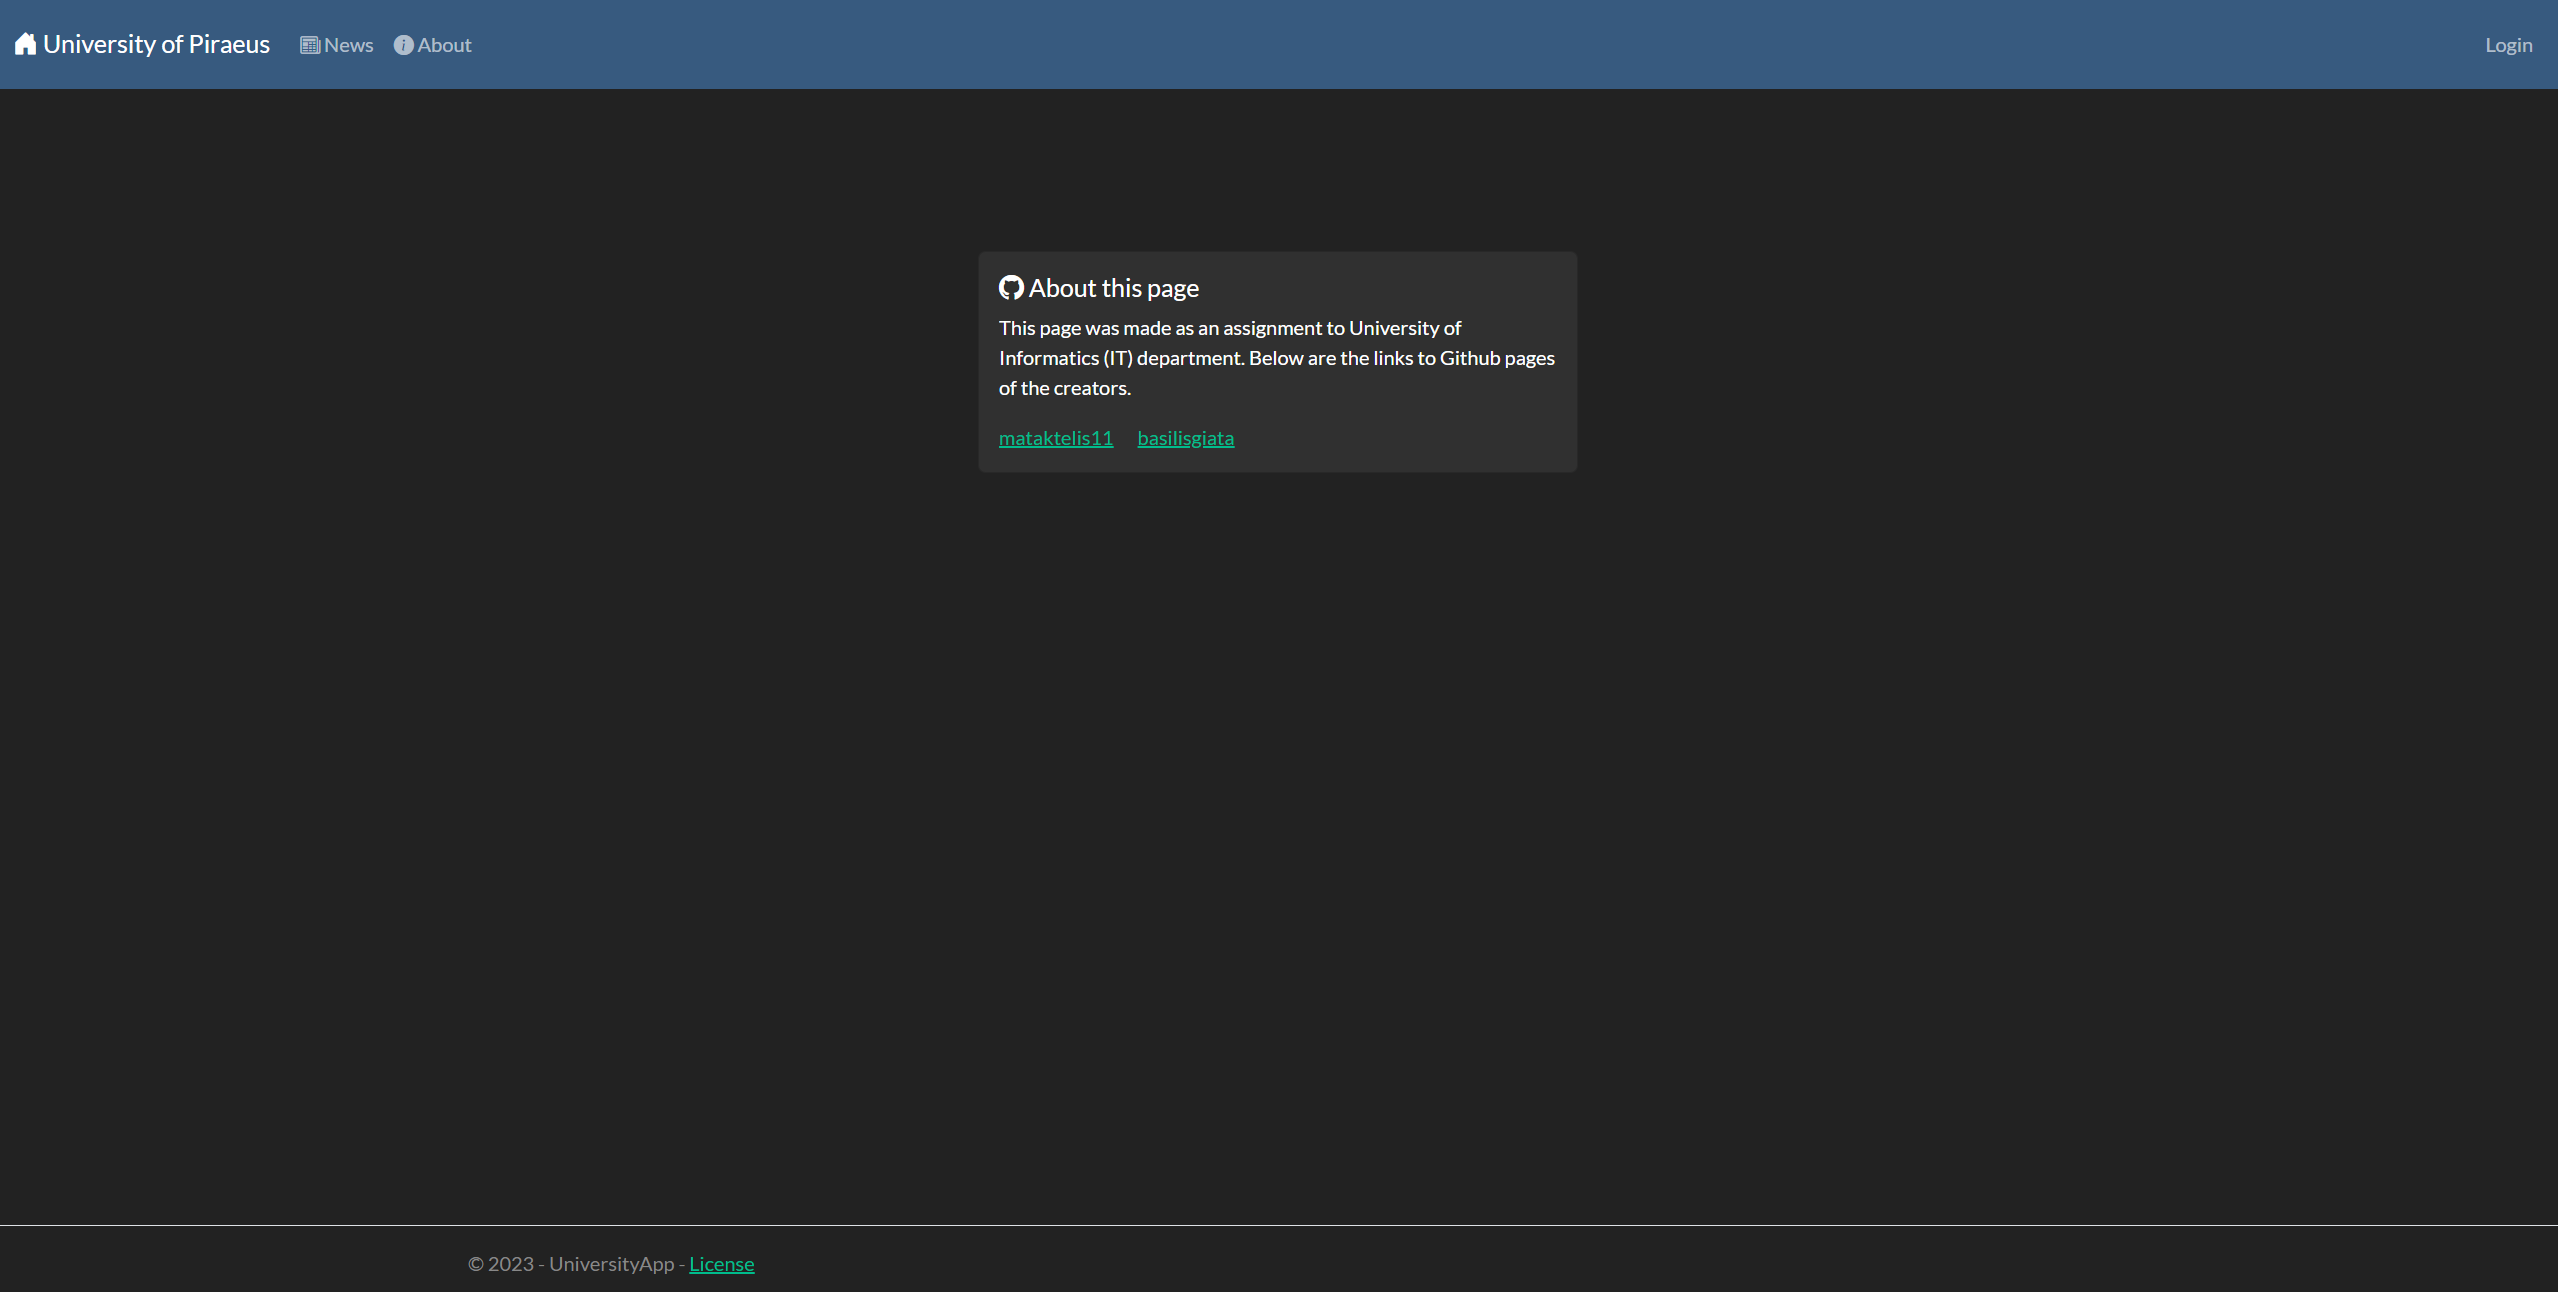
\includegraphics[width=0.85\textwidth]{abouts.png}
		\caption{About page}
		\label{fig:emptyView}
	\end{figure}

	Πατώντας στον σύνδεσμο 4 από το Nav bar (εικόνα \ref{fig:bar}) ο χρήστης θα μεταβεί στην παρακάτω ιστοσελίδα
	
	\begin{figure}[H]
	\centering
	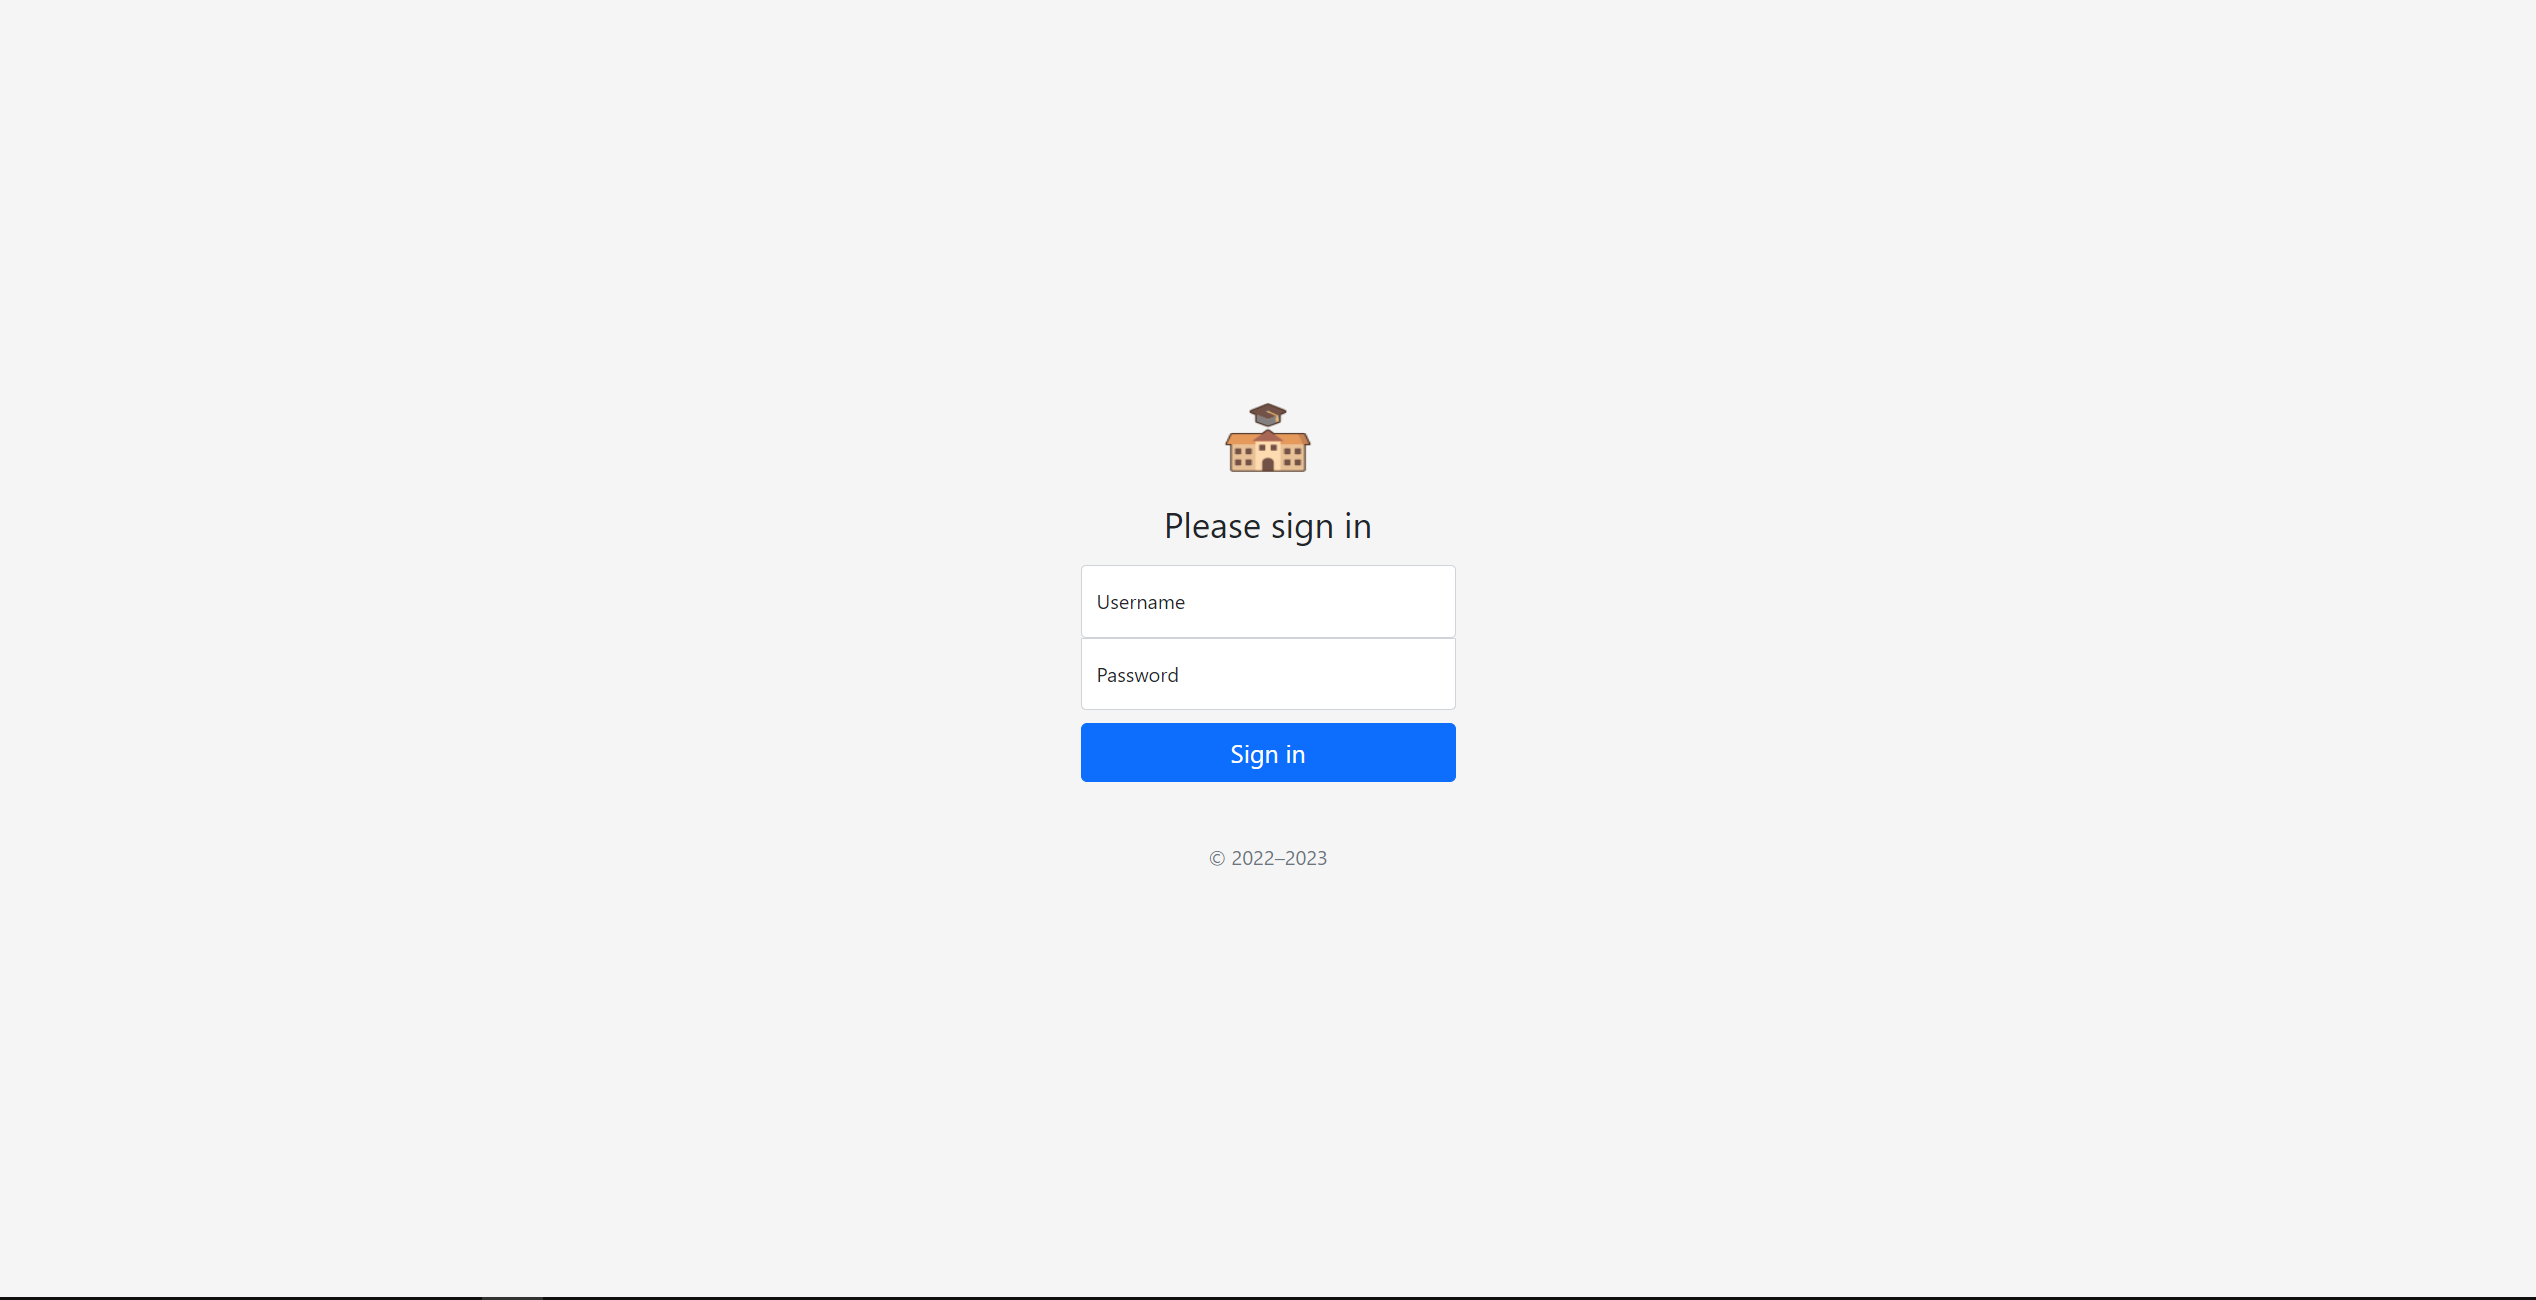
\includegraphics[width=0.85\textwidth]{logs.png}
	\caption{Log in page}
	\label{fig:emptyView}
	\end{figure}
	
	Εδώ θα συμπληρώσει το username και το password του και εφόσον είναι σωστά θα μεταβεί σε ιστοσελίδα ανάλογη με τον ρόλο του χρήστη στην Βάση Δεδομένων της εφαρμογής.
	
	Οι ιστοσελίδες και λειτουργίες που παρέχονται για τον κάθε ρόλο χρηστών περιγράφονται στις ξεχωριστές ενότητες που ακολουθούν.

	\newpage
	\subsection{Οδηγίες Φοιτητών}
	
	Όταν ο φοιτητής δώσει τους σωστούς κωδικούς του θα μεταβεί στην παρακάτω σελίδα καλωσόρισης. Ενδεικτικά δίνονται τα παρακάτω credetials:
	
	\begin{itemize}
		\item Username : \textbf{jibbesonu}
		\item Password : \textbf{pFVJ4ra}
	\end{itemize}



	\begin{figure}[H]
	\centering
	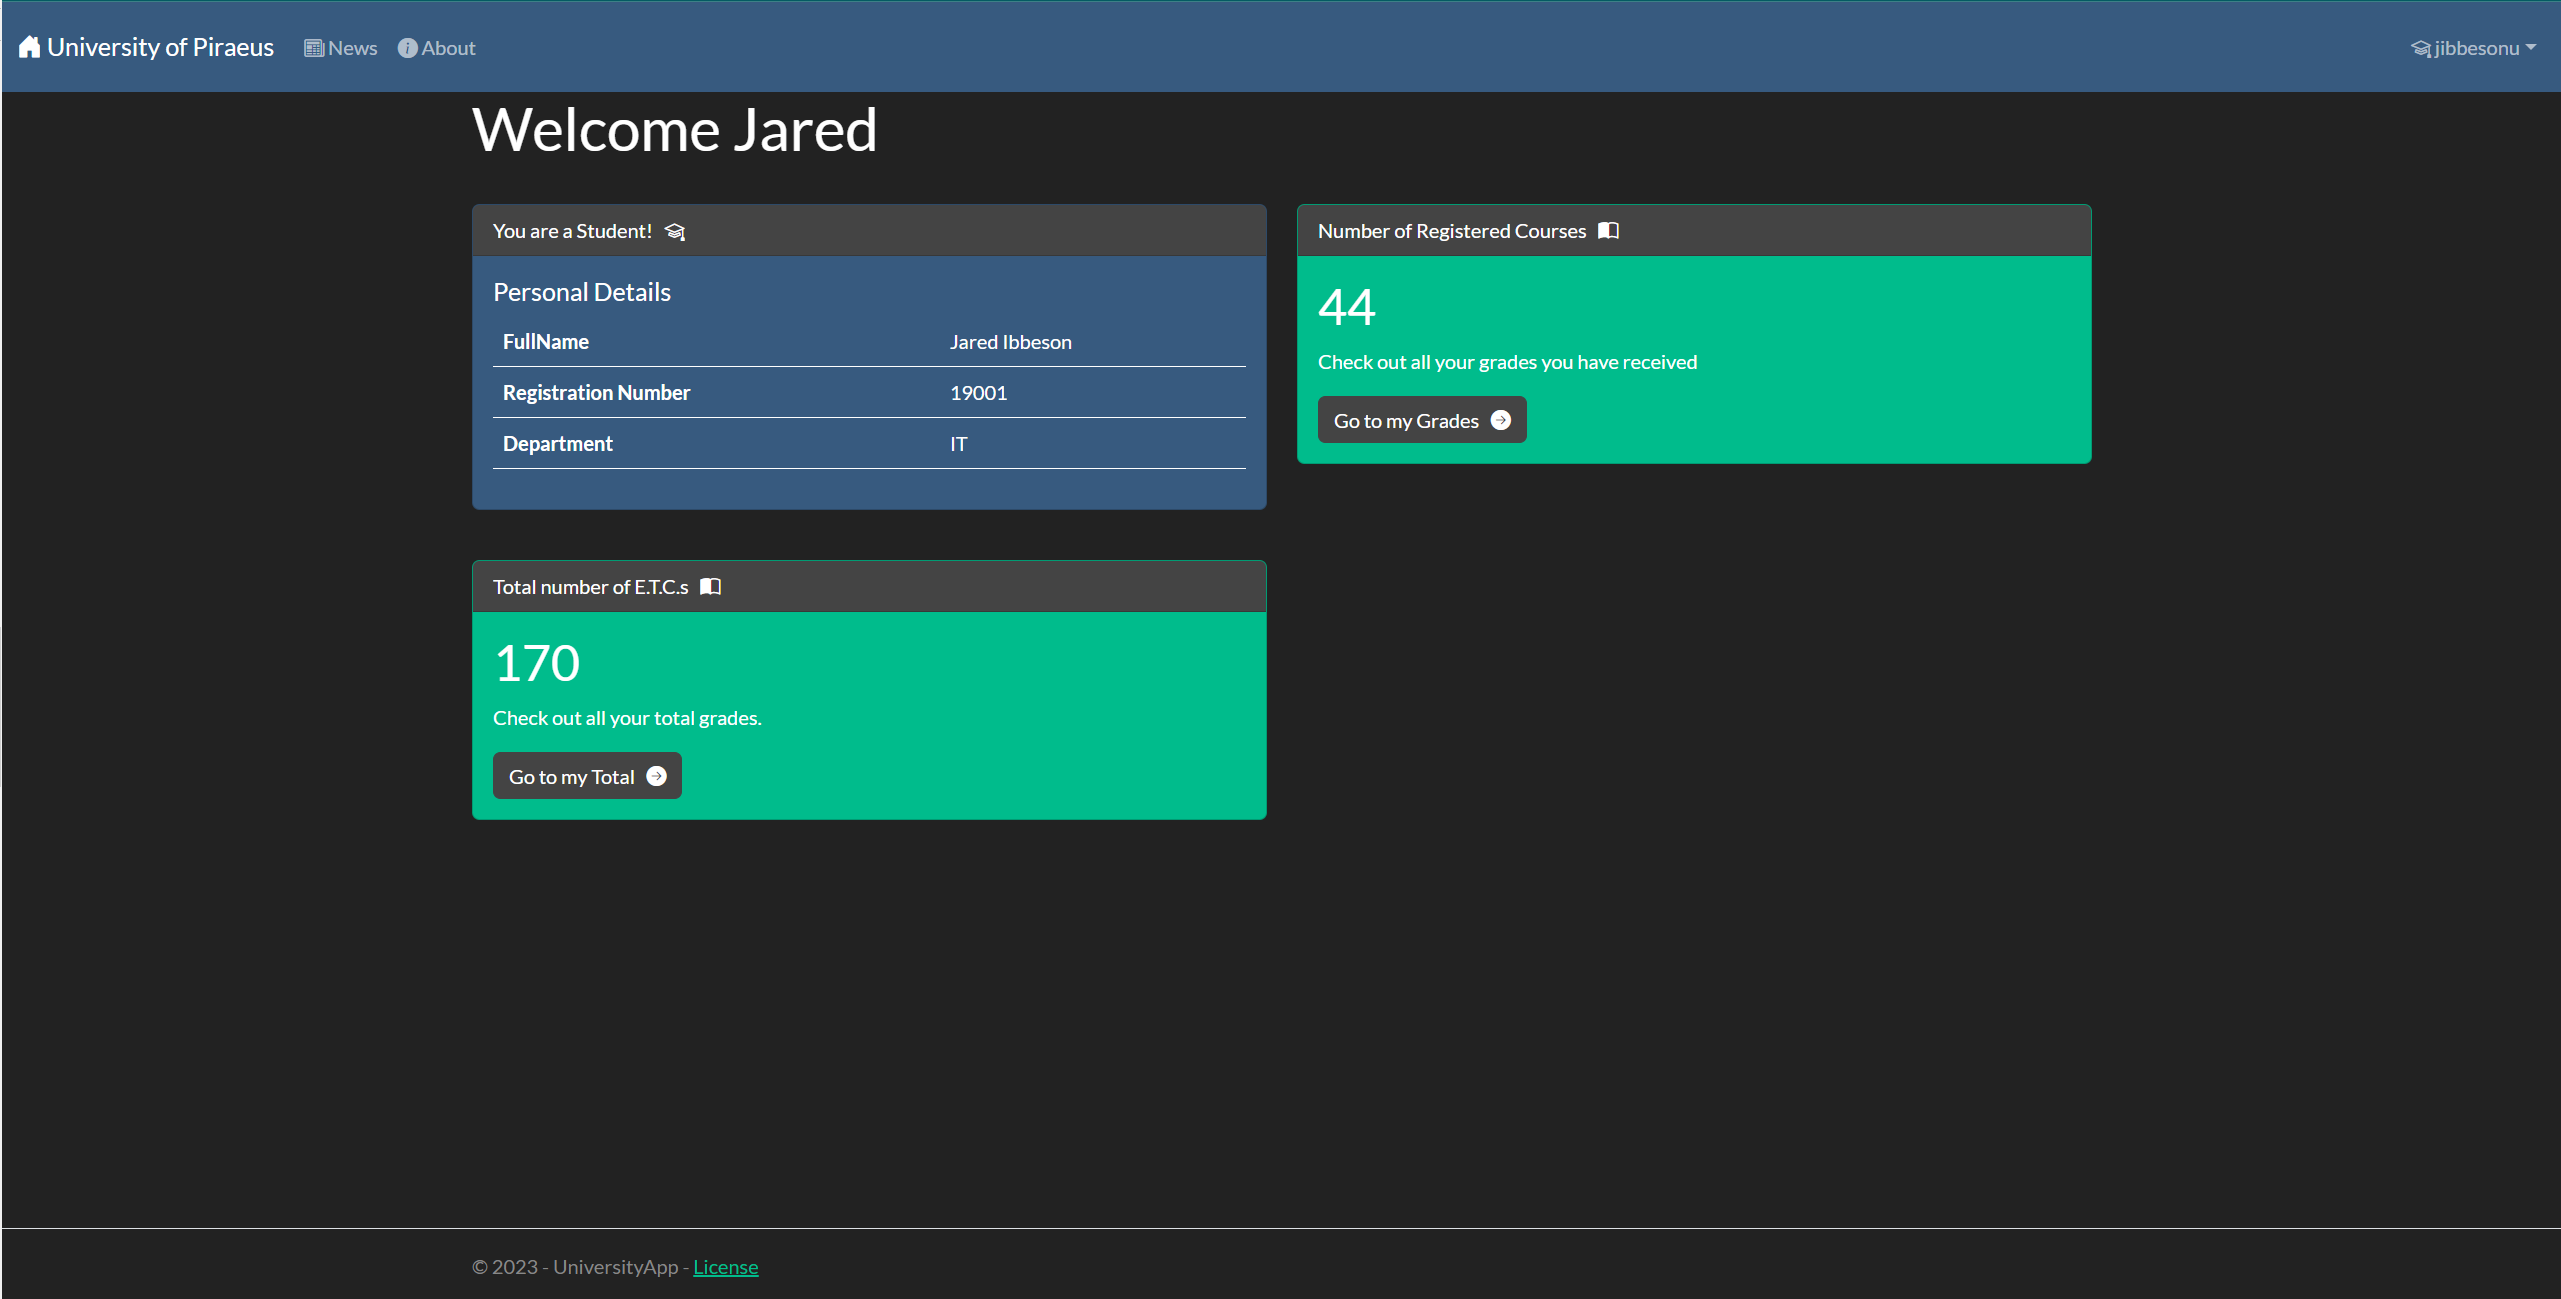
\includegraphics[width=0.85\textwidth]{studentwel.png}
	\caption{Student welcome page}
	\label{fig:emptyView}
	\end{figure}

	Εδώ περιέχονται τα στοιχεία του και σύντομες πληροφορίες για αυτόν όπως ο αριθμός δηλωμένων μαθημάτων () και ο αριθμός των E.C.T.s που έχει (). Υπάρχουν επίσης σύνδεσμοι που κατευθύνουν τον φοιτητή στη σελίδα των βαθμολογιών του () και στην σελίδα των συνολικών βαθμολογιών του αντίστοιχα (). Οι επιλογές αυτές είναι διαθέσιμες και στο μενού που εμφανίστηκε στο δεξί μέρος της μπάρας της σελίδας.
	
	Αν ο φοιτητής επιλέξει να μεταβεί στην σελίδα των βαθμολογιών του είτε μέσω του μενού είτε από τον σύνδεσμο της αρχικής σελίδας, η εφαρμογή θα εμφανίσει την παρακάτω σελίδα.
	
	\begin{figure}[H]
		\centering
		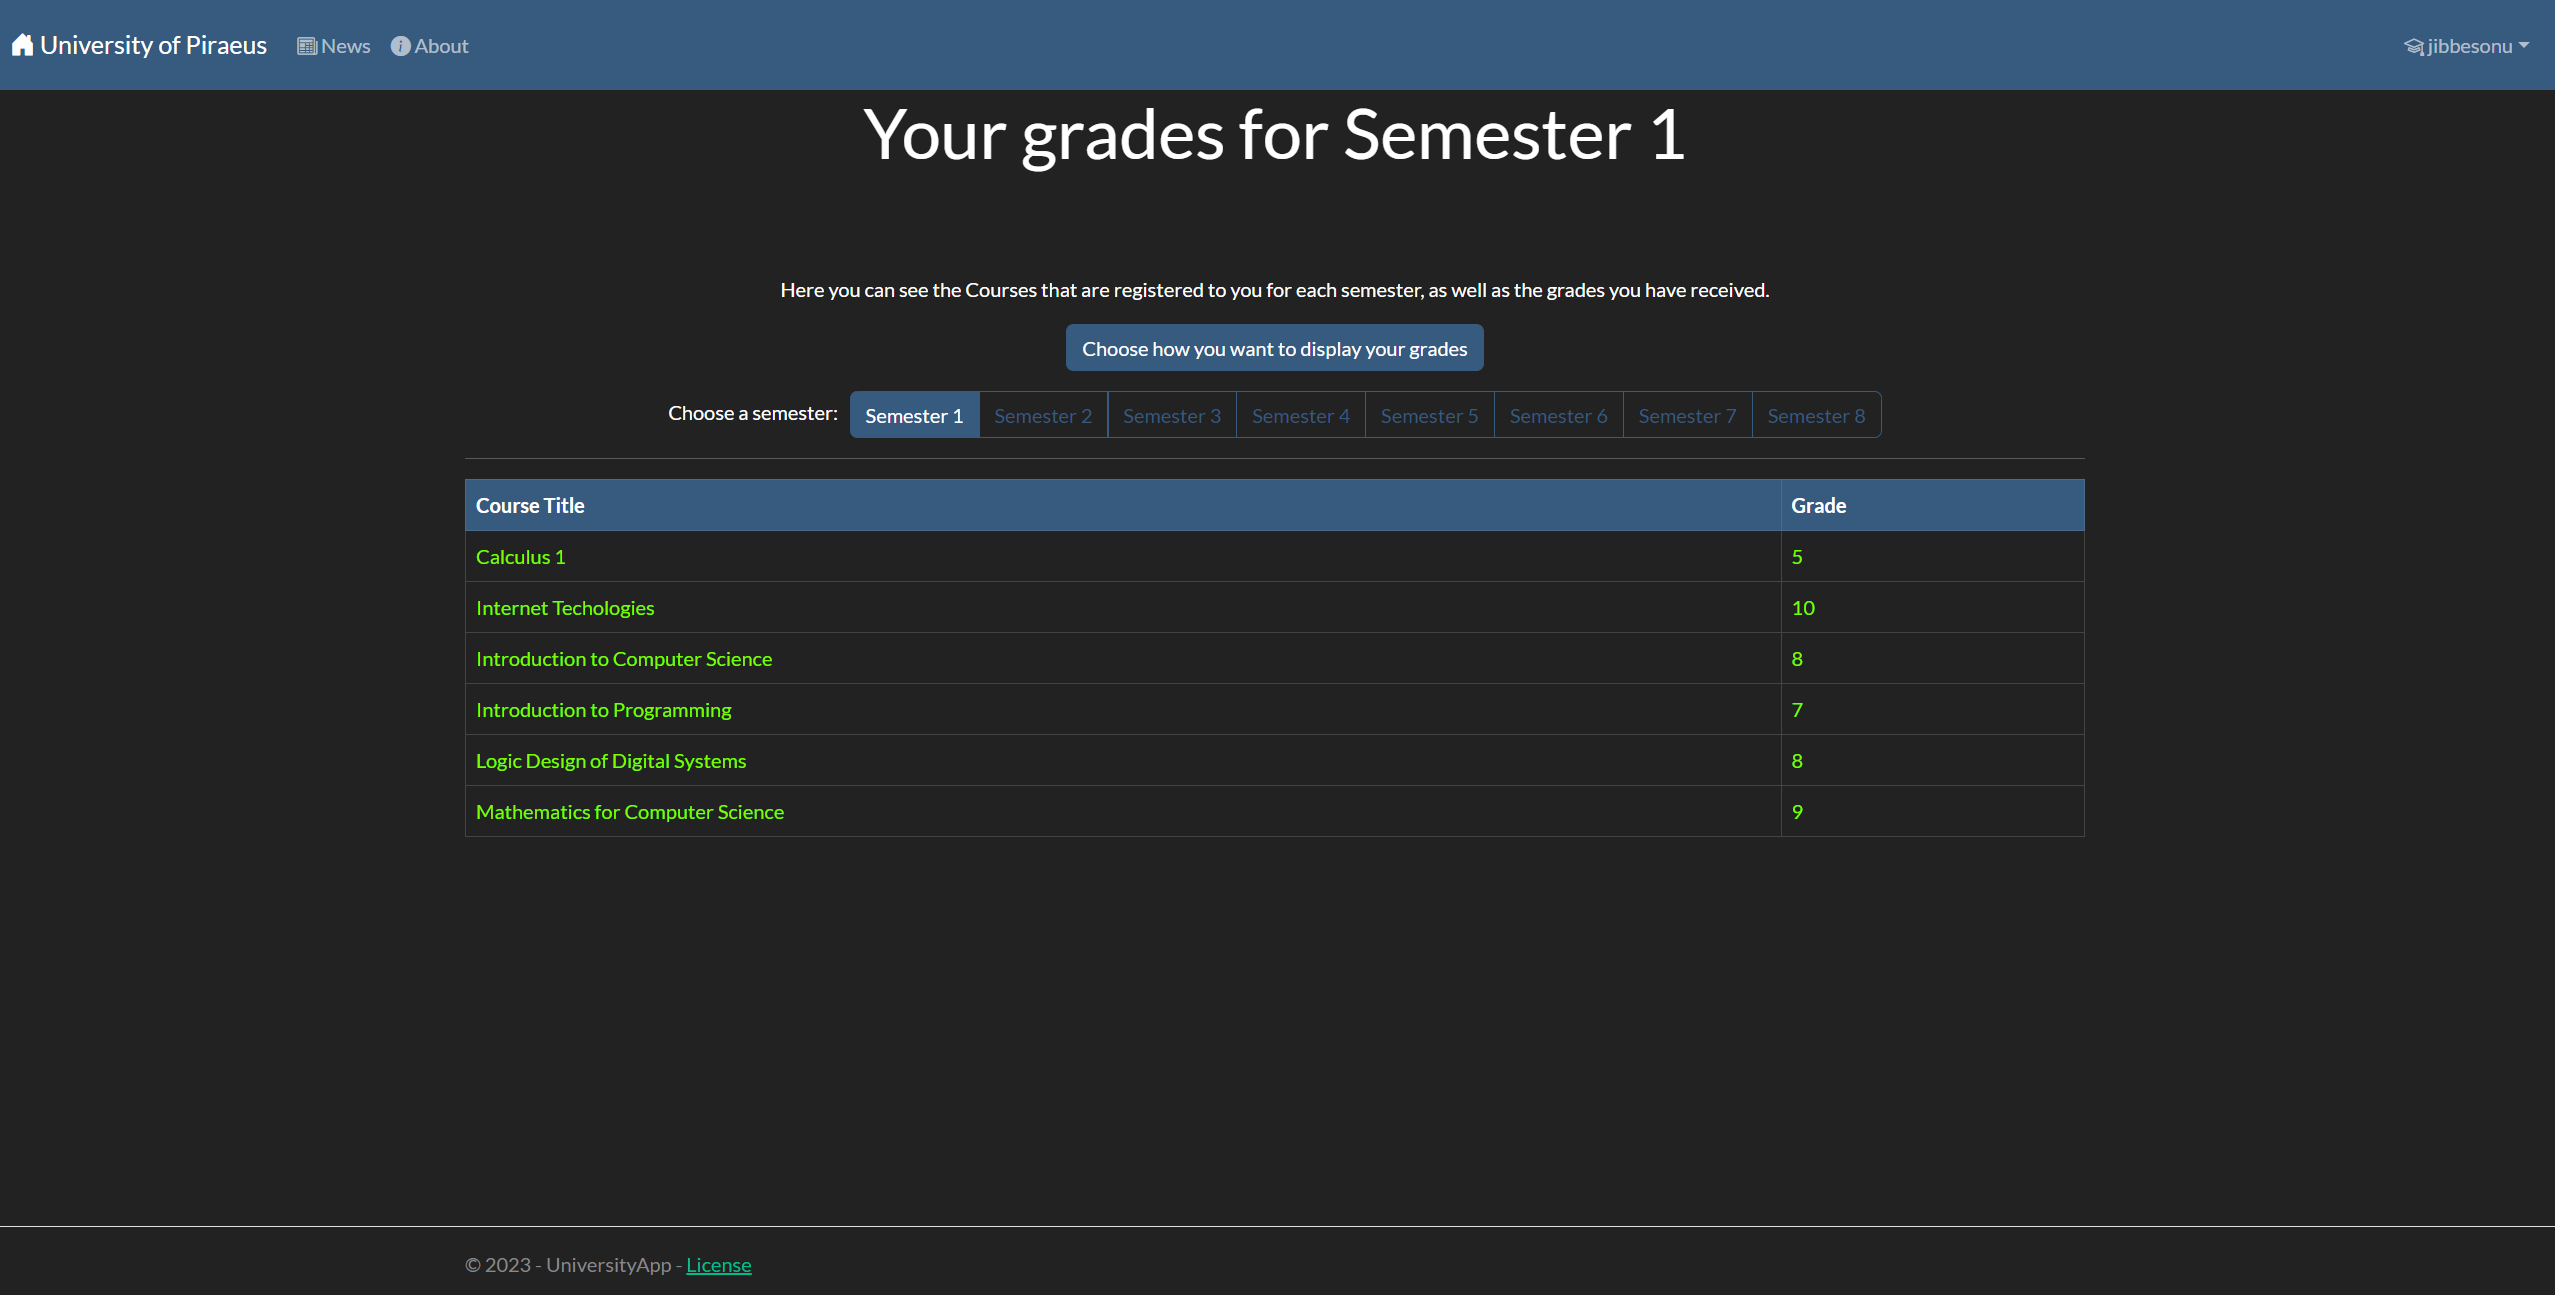
\includegraphics[width=0.85\textwidth]{semesters1.png}
		\caption{Student Semesters page}
		\label{fig:emptyView}
	\end{figure}
	
	Εδώ ο φοιτητής βλέπει τα μαθήματα που έχει δηλωμένα στο πρώτο εξάμηνο καθώς και τον βαθμό για το κάθε μάθημα. Ο φοιτητής μπορεί να κάνει κλικ πάνω στα κουμπιά με την ένδειξη 'Semesters' ώστε να επιλέξει το εξάμηνο που επιθυμεί.
	
	Αν το εξάμηνο που επιλέχθηκε από τον φοιτητή δεν περιέχει κανένα μάθημα τότε θα εμφανιστεί ένα κατάλληλο μήνυμα και μία εικόνα.
	
	\begin{figure}[H]
		\centering
		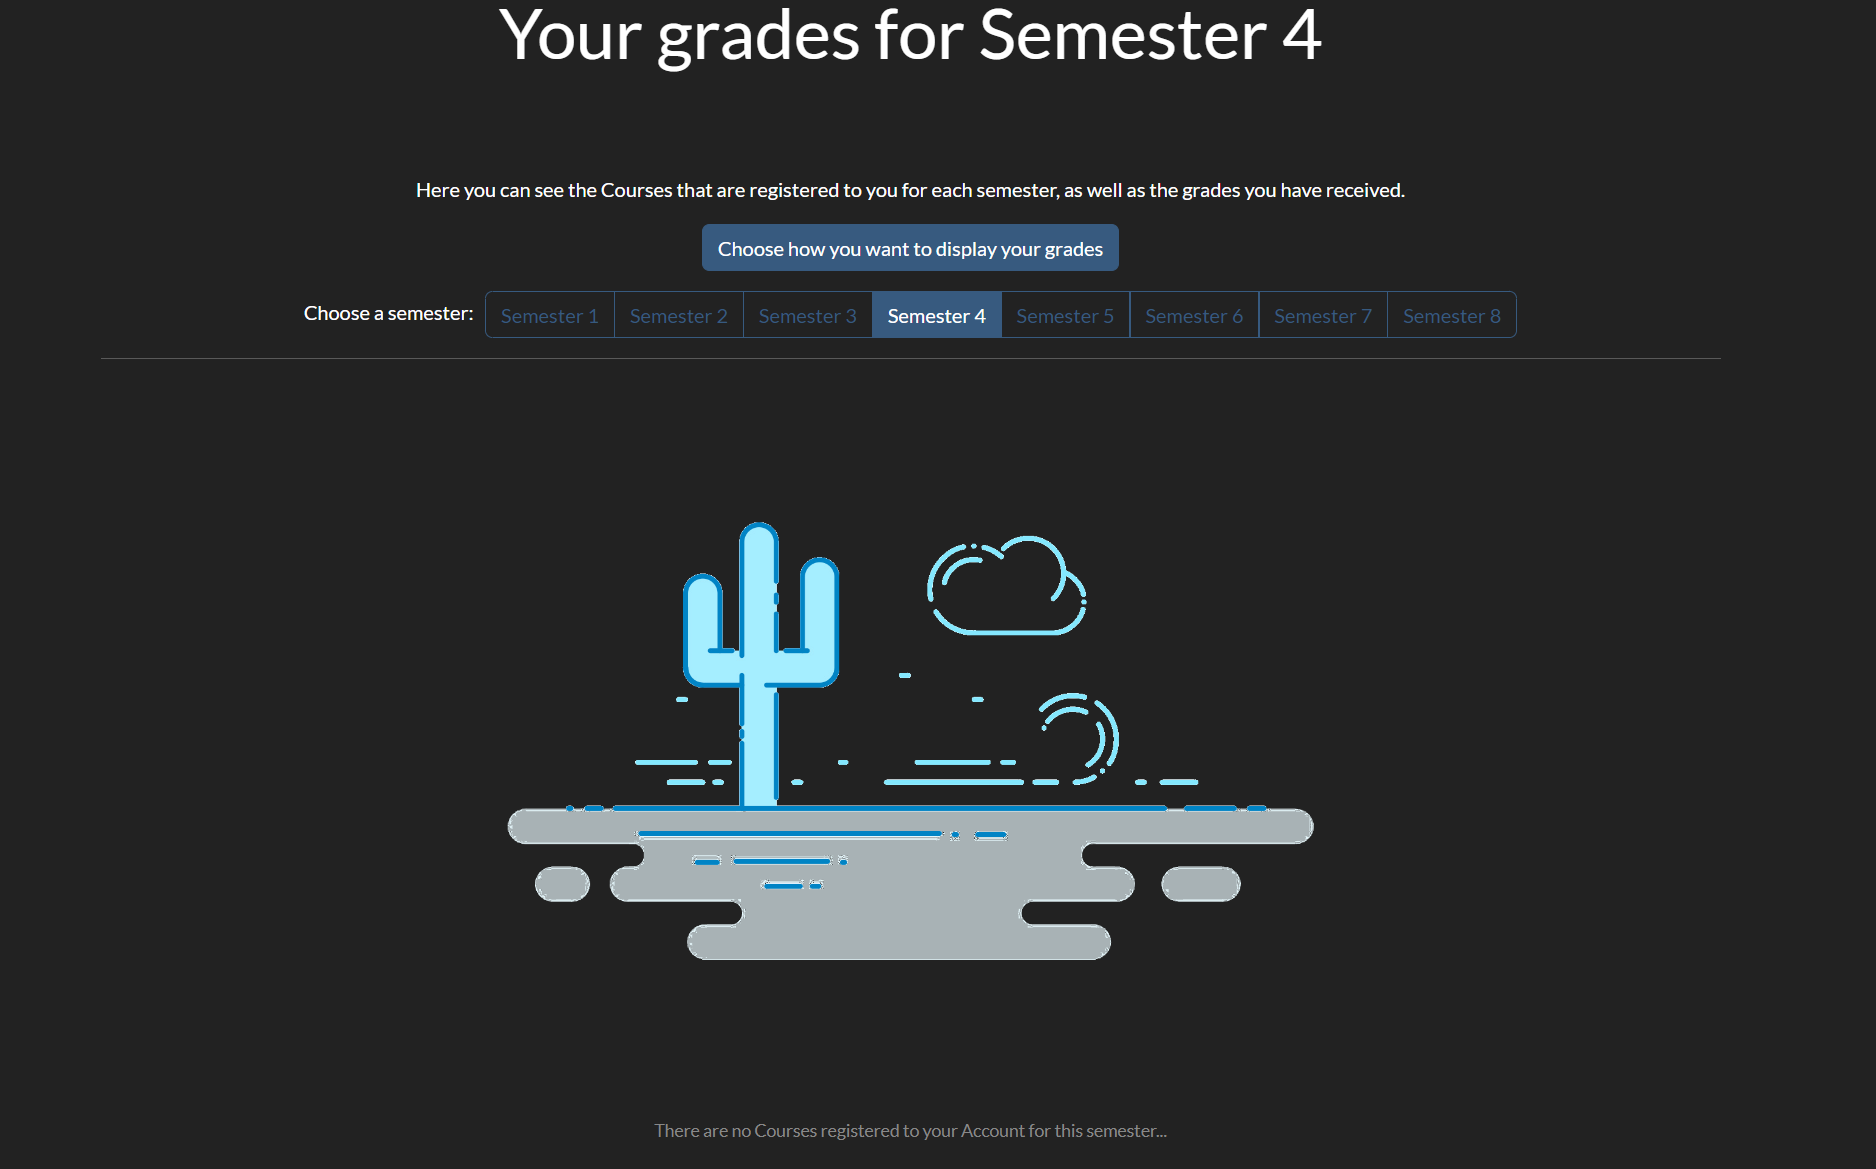
\includegraphics[width=0.85\textwidth]{nolessons.png}
		\caption{Παράδειγμα εξαμήνου που δεν υπάρχει δηλωμένο μάθημα}
		\label{fig:emptyView}
	\end{figure}
	
	Υπάρχει επιπλέον η επιλογή '\textbf{Choose how you want to display your grades}' με την οποία εμφανίζεται ένα μενού στα αριστερά της σελίδας.

	\begin{figure}[H]
		\centering
		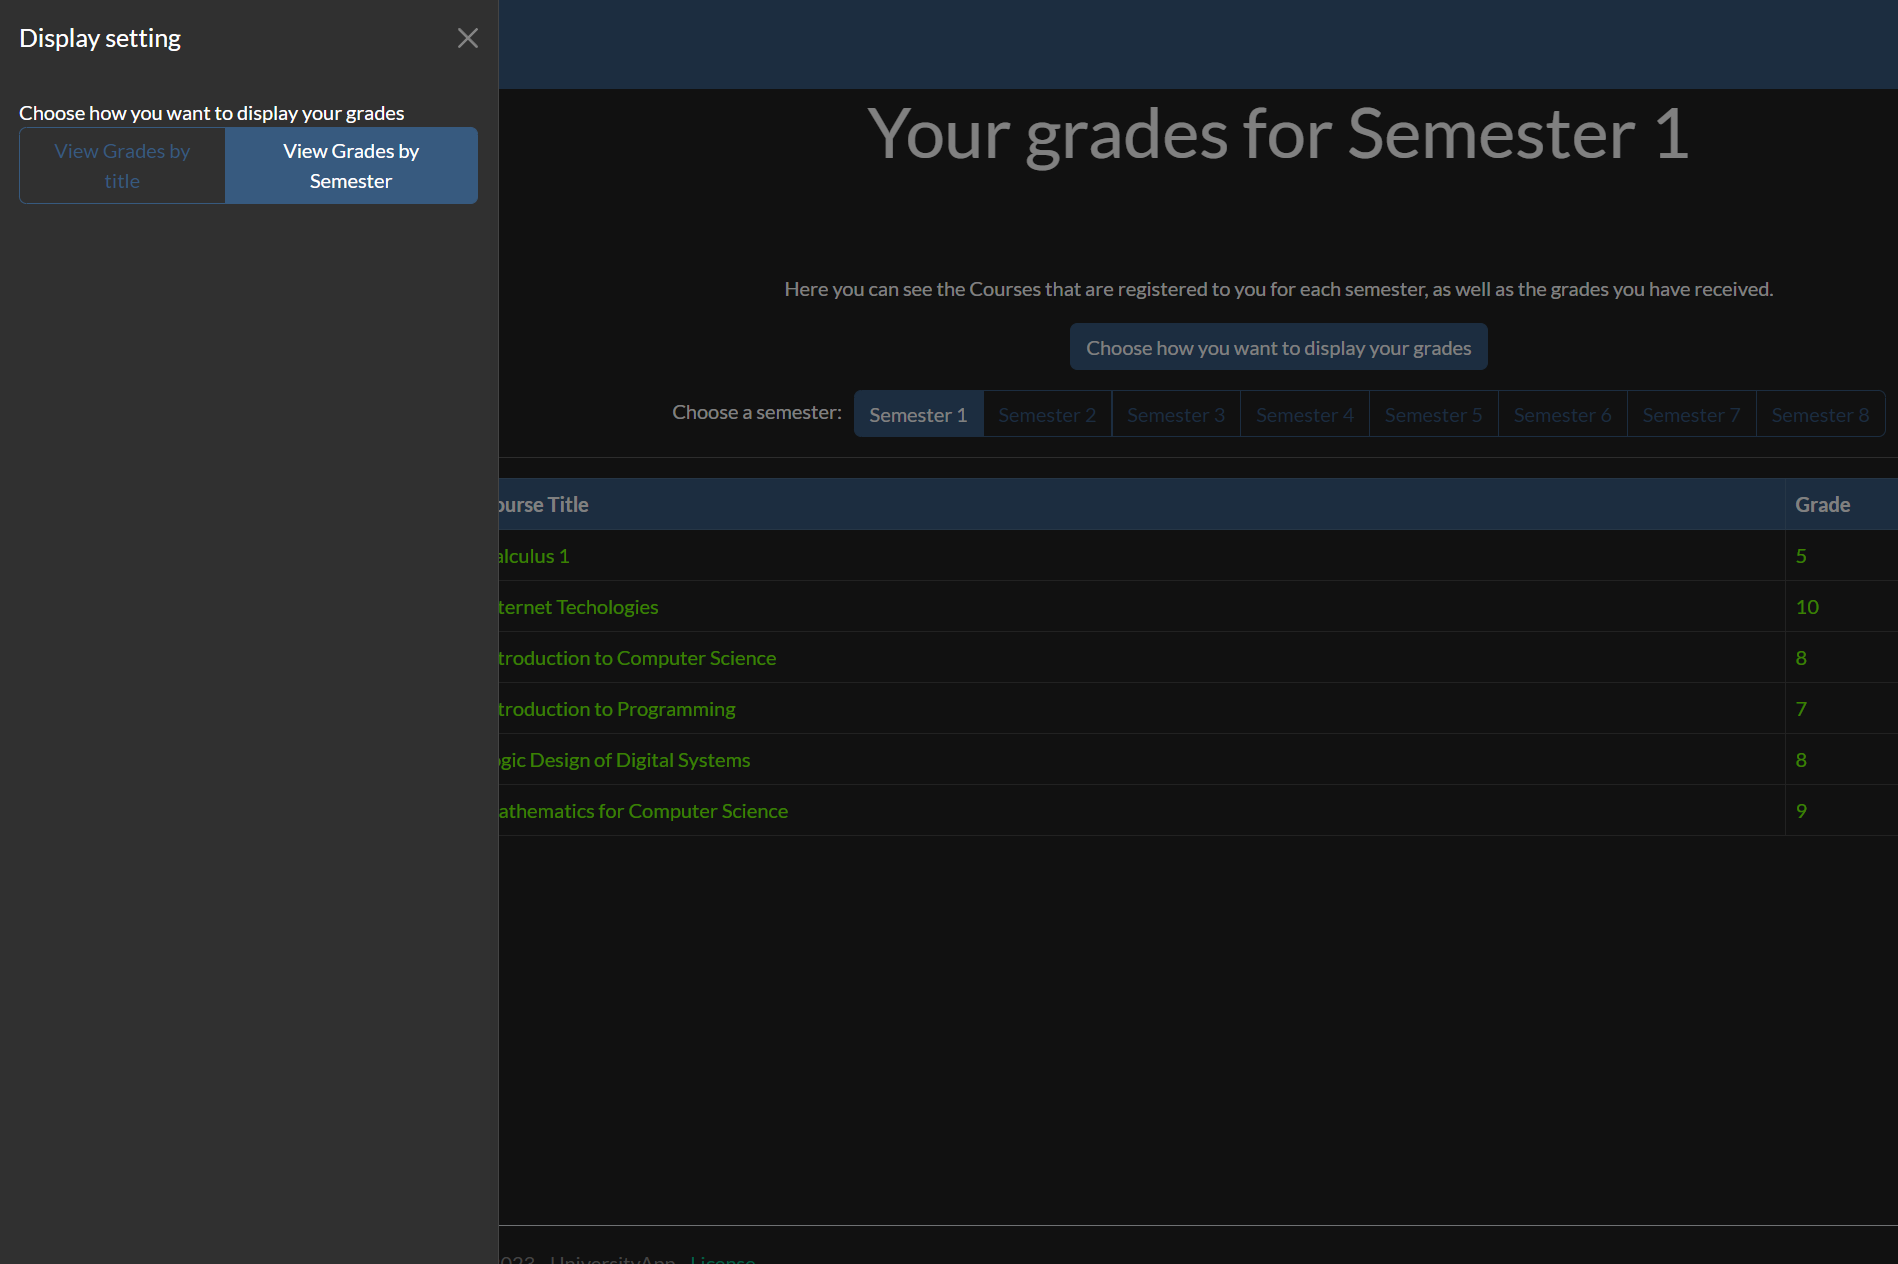
\includegraphics[width=0.85\textwidth]{sidemenu.png}
		\caption{Side menu}
		\label{fig:emptyView}
	\end{figure}	
	
	Εδώ ο φοιτητής μπορεί να επιλέξει πώς θέλει να εμφανιστούν οι βαθμοί του. Τώρα είναι επιλεγμένη η επιλογή 'View grades by semester'. Αν ο φοιτητής επιλέξει την δεύτερη διαθέσιμη επιλογή η σελίδα των βαθμολογιών θα αλλάξει όπως φαίνεται παρακάτω.
	
	\begin{figure}[H]
	\centering
	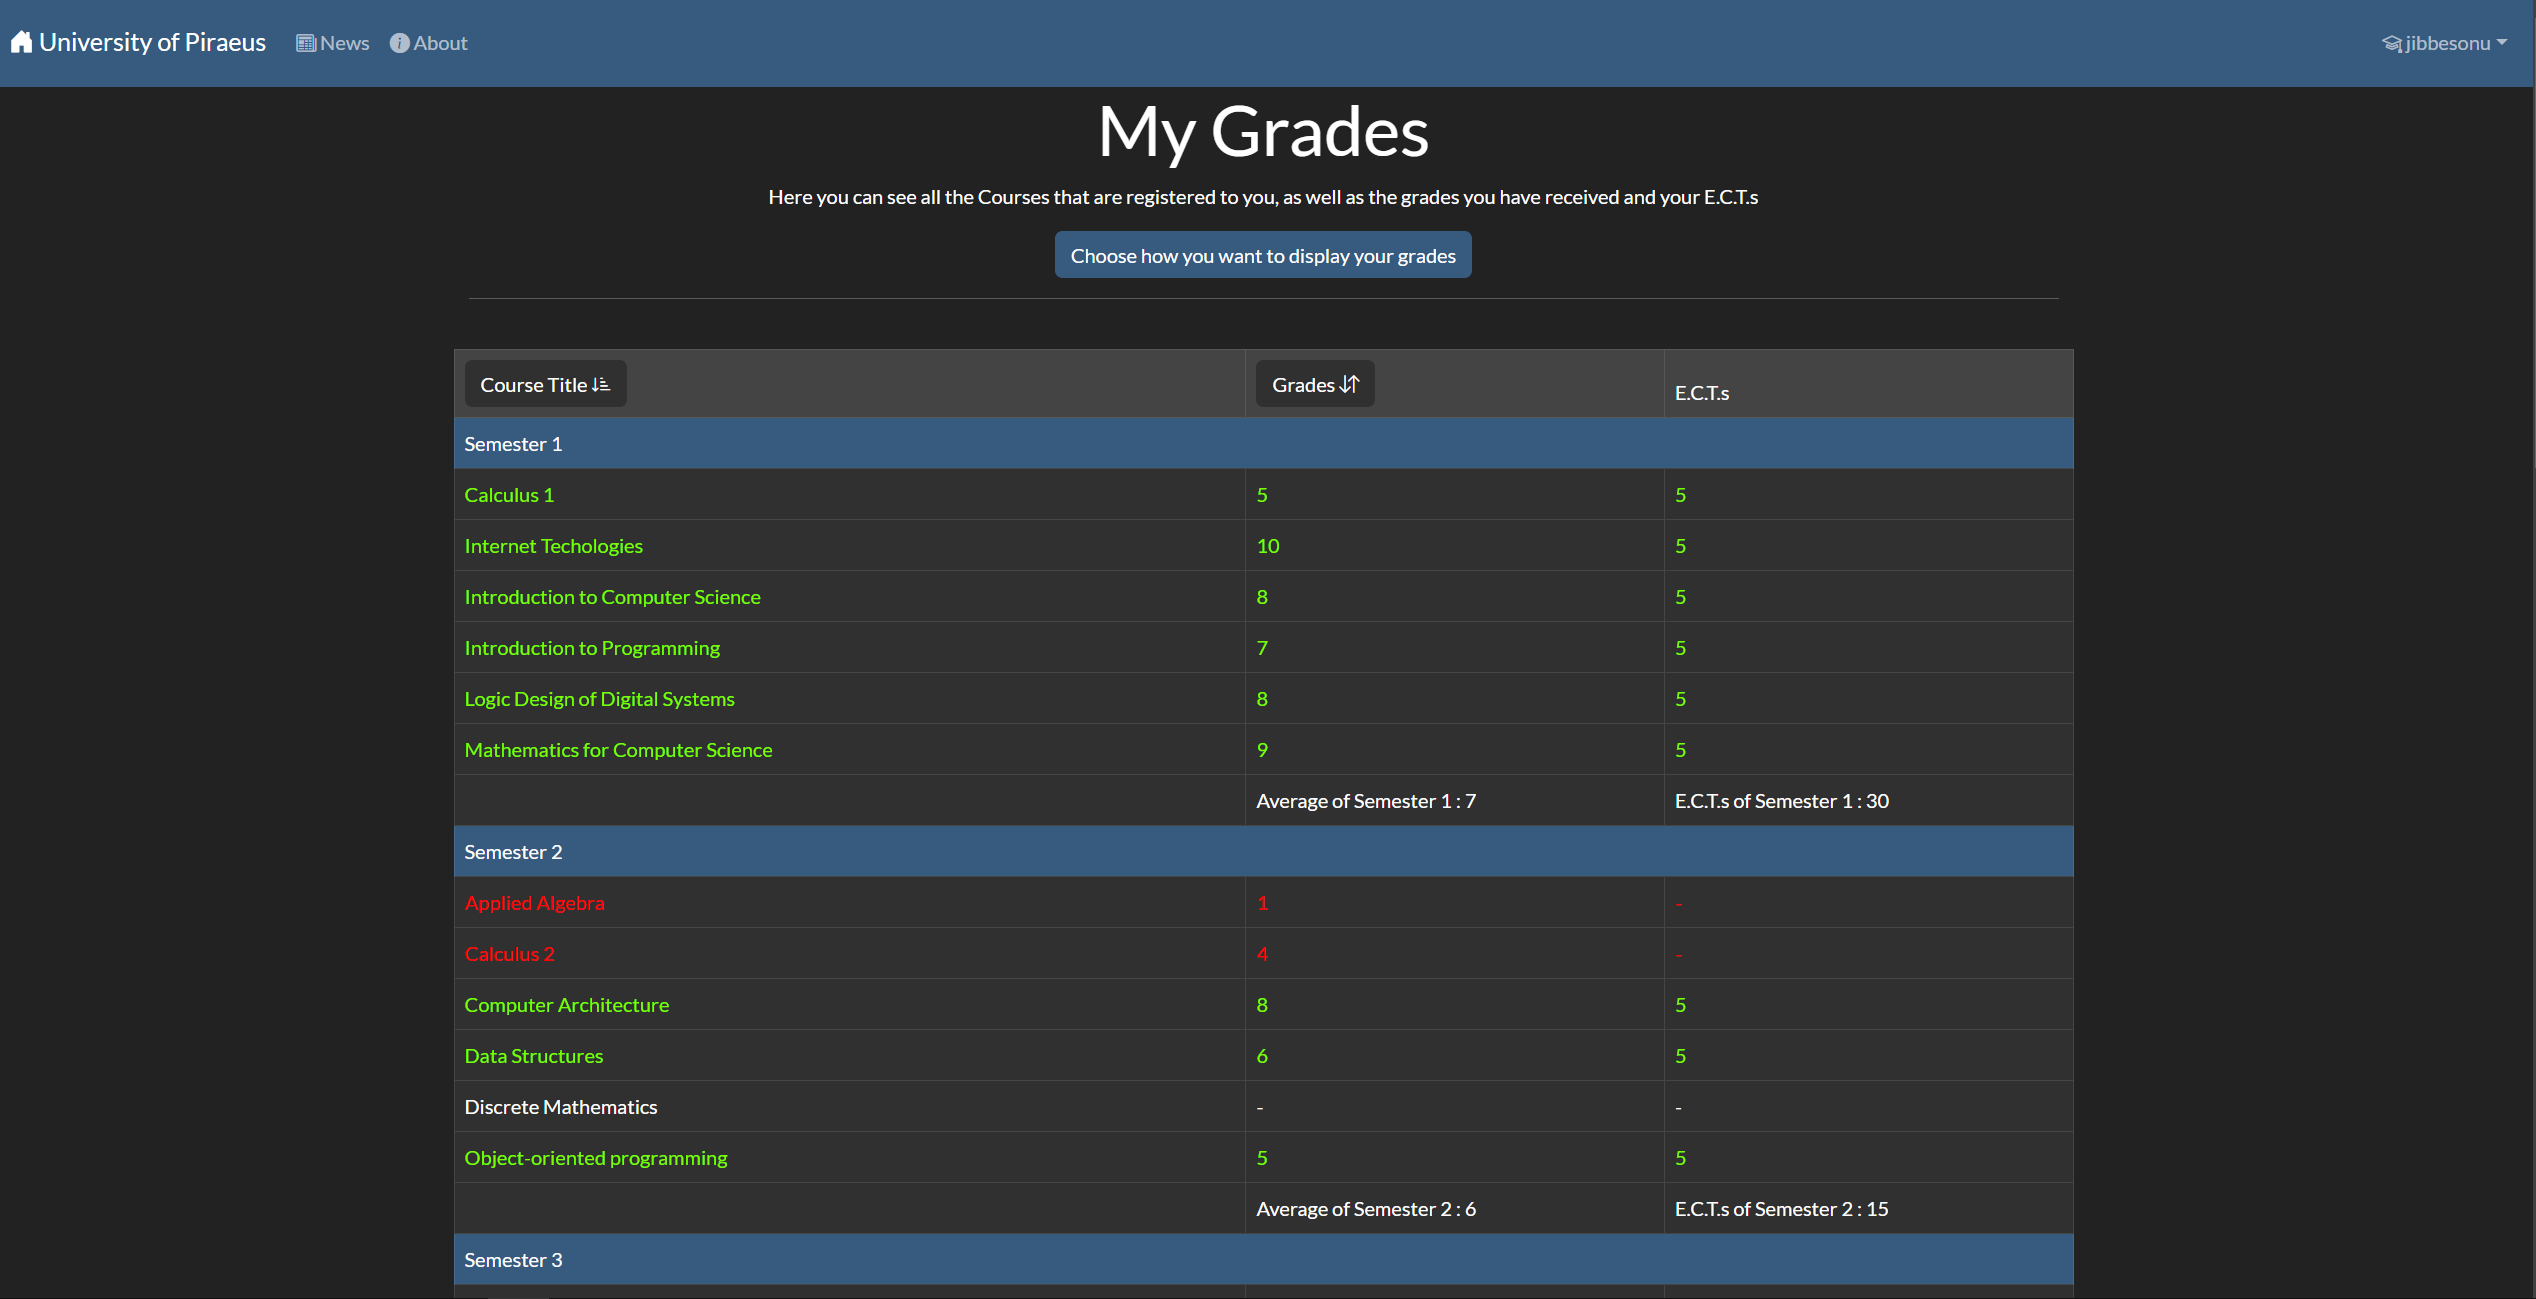
\includegraphics[width=0.85\textwidth]{allgrades.png}
	\caption{}
	\label{fig:emptyView}
	\end{figure}

	Στο τέλος κάθε εξαμήνου φαίνεται το σύνολο των E.C.T.s και ο μέσος όρος για το εξάμηνο. Στο τέλος της σελίδας φαίνεται ο συνολικός μέσος όρος και τα συνολικά E.C.T.s.
	
	Σε αυτή τη σελίδα περιλαμβάνονται όλα τα εξάμηνα με τα αντίστοιχα μαθήματα και τις βαθμολογίες. Ο φοιτητής μπορεί να πατήσει στο κουμπί με την ίδια ένδειξη () αν θέλει να εμφανίσει πάλι το μενού και να επαναφέρει την προηγούμενη σελίδα βαθμολογιών
		

	\newpage
	\subsection{Οδηγίες Καθηγητών}
	
	Όταν ο καθηγητής δώσει τους σωστούς κωδικούς του θα μεταβεί στην παρακάτω σελίδα καλωσόρισης. Ενδεικτικά δίνονται τα παρακάτω credetials:
	
	\begin{itemize}
		\item Username : \textbf{cbococka}
		\item Password : \textbf{Sc5GIg}
	\end{itemize}

	\begin{figure}[H]
	\centering
	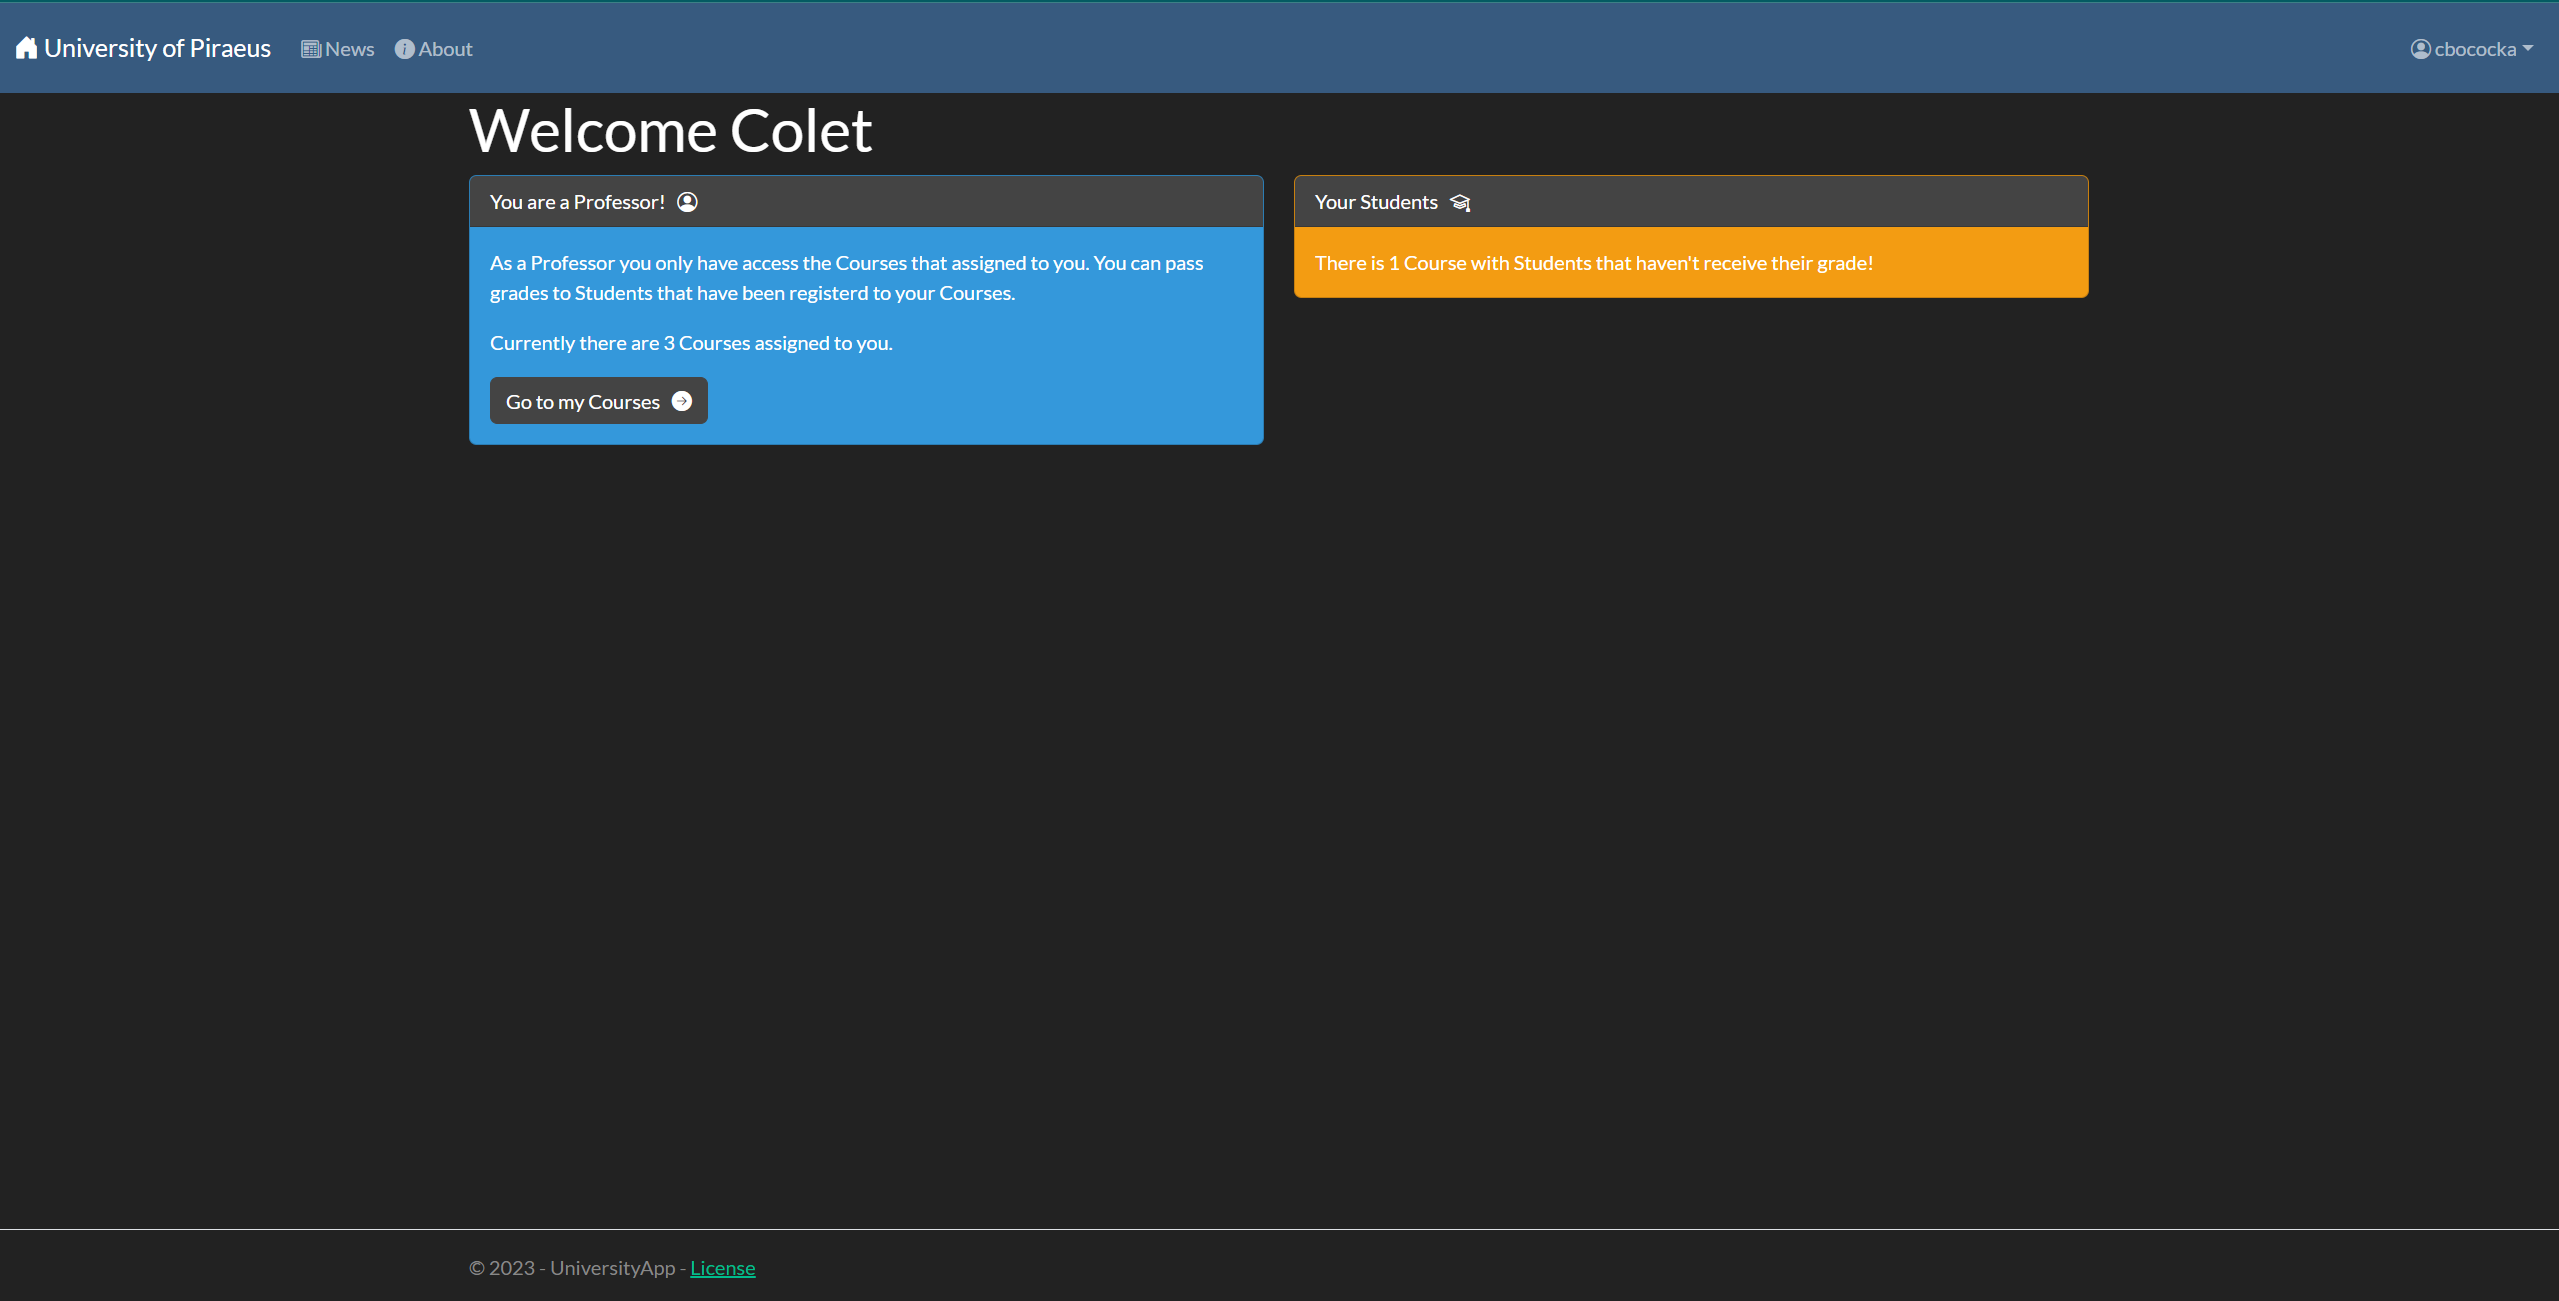
\includegraphics[width=0.85\textwidth]{wellprof.png}
	\caption{}
	\label{fig:emptyView}
	\end{figure}

	Η σελίδα καλωσόρισης του καθηγητή περιέχει 3 κάρτες. Στην κάρτα () φαίνεται αν υπάρχουν μαθήματα για τα οποία δηλωμένοι φοιτητές δεν έχουν λάβει βαθμό. Αν ο καθηγητής επιλέξει να μεταβεί στην σελίδα των βαθμολογιών του είτε μέσω του μενού είτε από τον σύνδεσμο της αρχικής σελίδας, η εφαρμογή θα εμφανίσει την παρακάτω σελίδα.
	
	\begin{figure}[H]
		\centering
		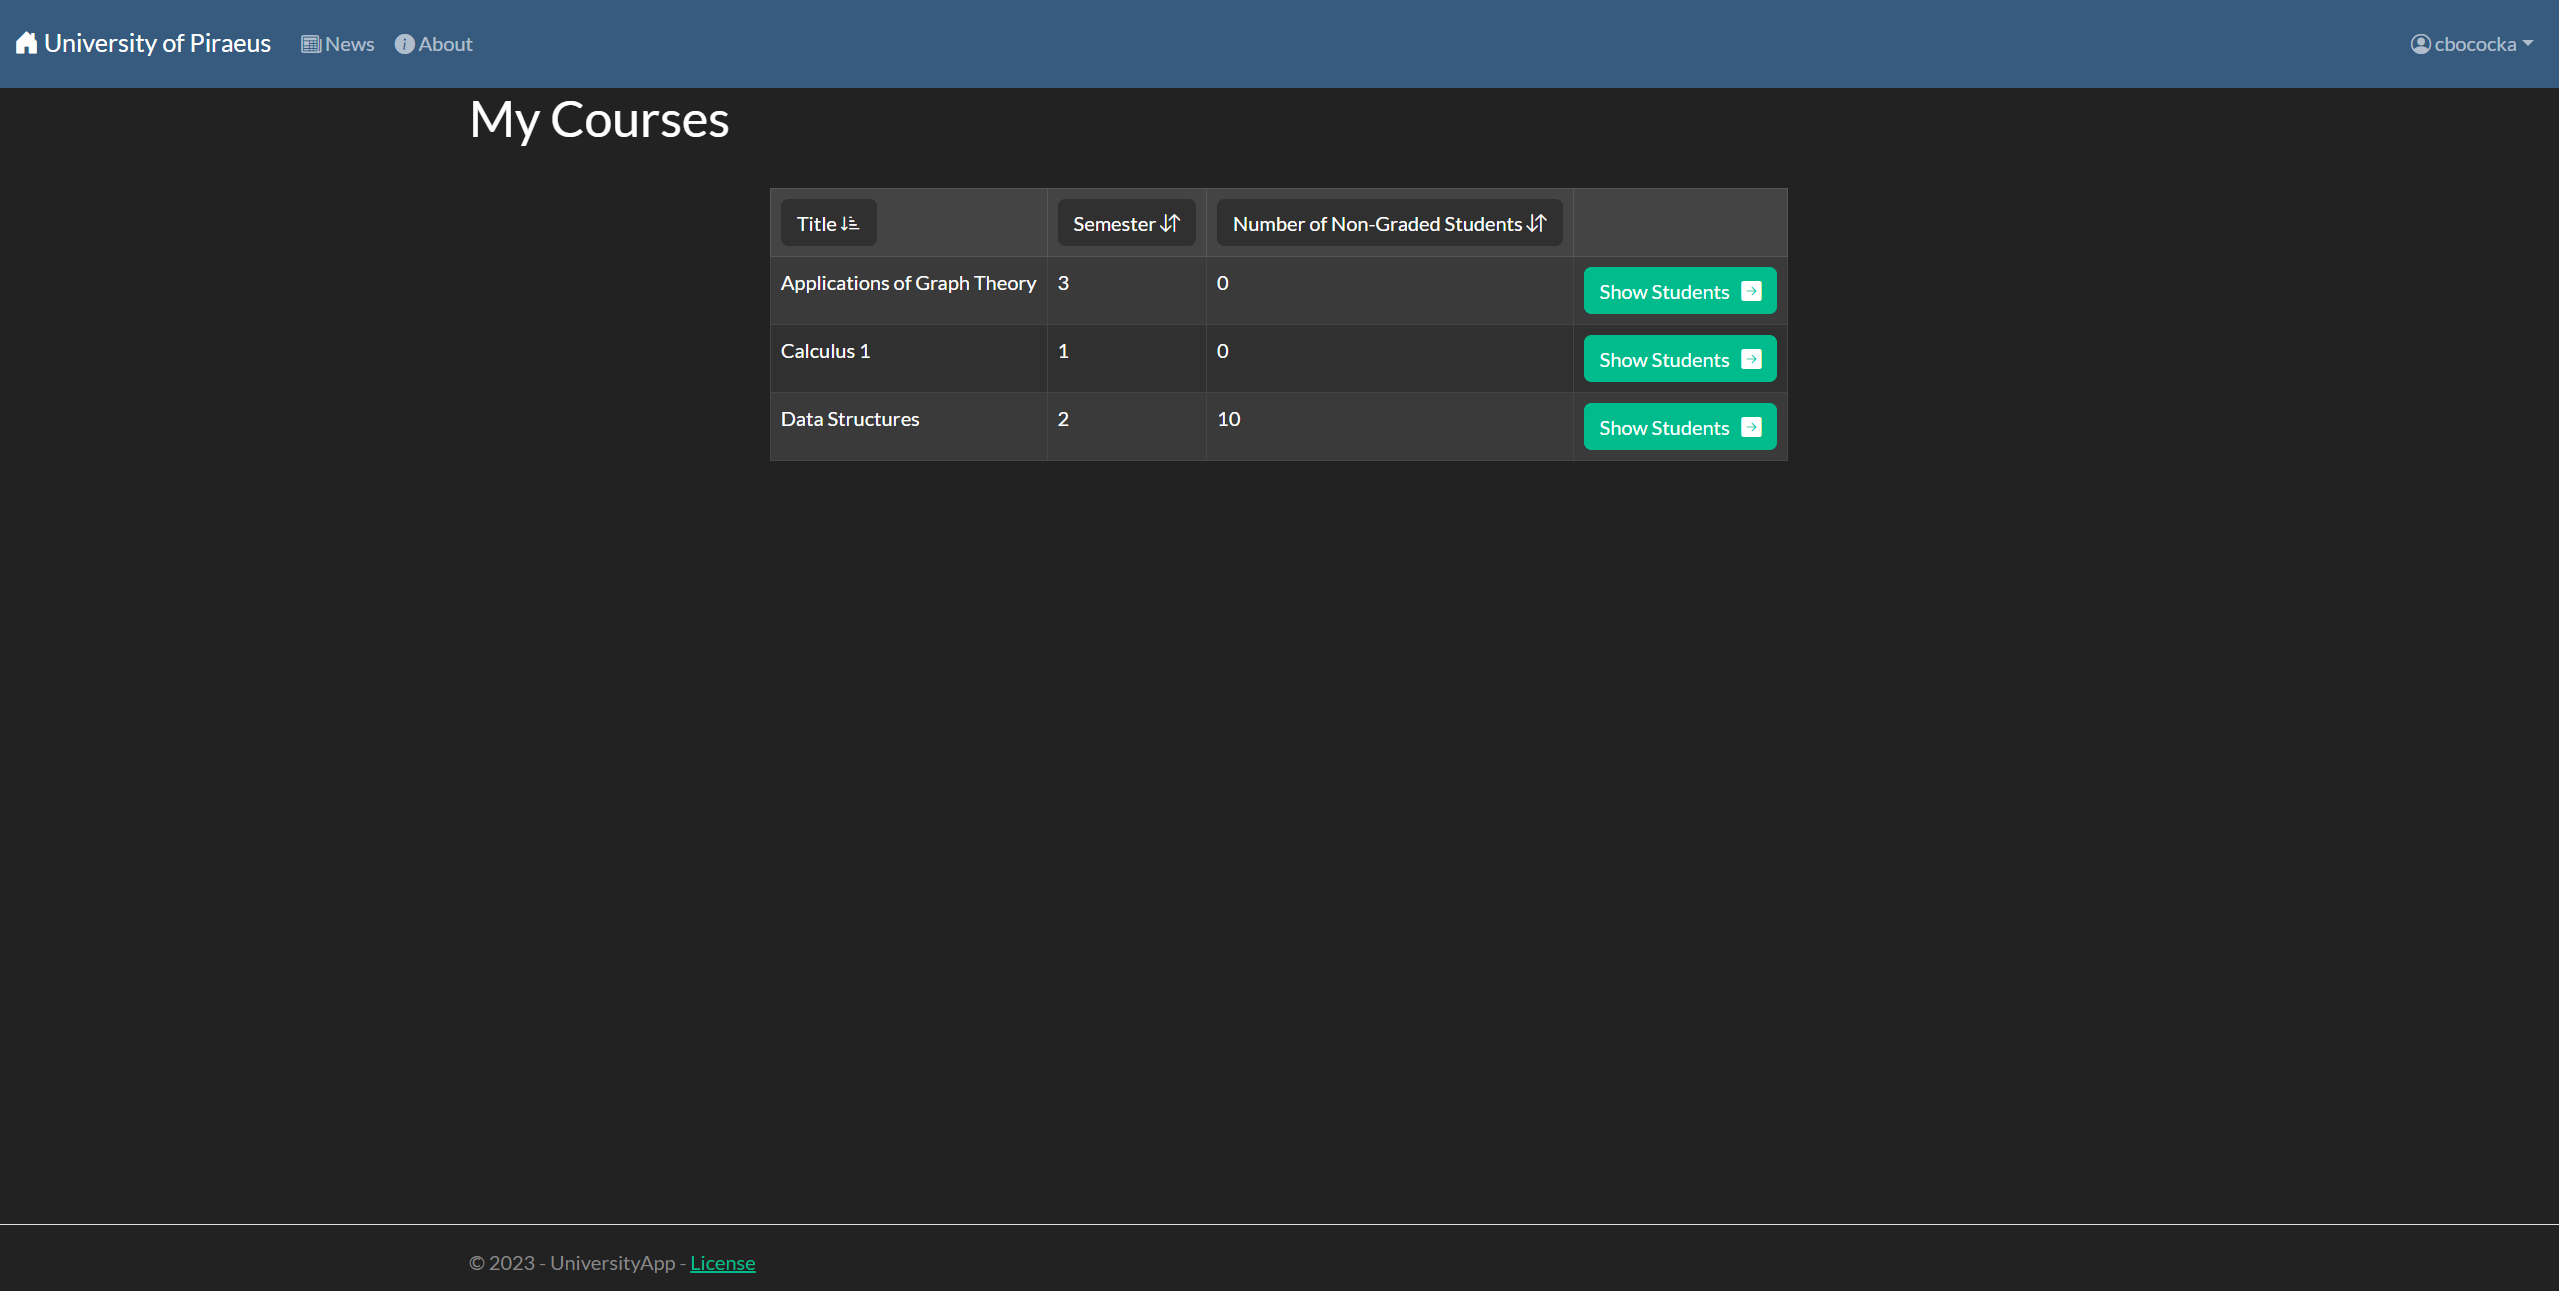
\includegraphics[width=0.85\textwidth]{mylessons.png}
		\caption{}
		\label{fig:emptyView}
	\end{figure}
	
	Σε αυτή τη σελίδα υπάρχουν όλα τα μαθήματα τα οποία έχουν ανατεθεί στον καθηγητή σε έναν πίνακα. Για κάθε μάθημα στη λίστα εμφανίζεται ο αριθμός των δηλωμένων Φοιτητών που δεν έχουν λάβει βαθμό. ο καθηγητής έχει την επιλογή να ταξινομήσει τον πίνακα ως προς οποιαδήποτε από τις 2 στήλες πατώντας στην επικεφαλίδα της κάθε λίστας.
	
	Επιλέγοντας ένα μάθημα ο καθηγητής θα μεταβεί στη σελίδα του μαθήματος όπου φαίνονται όλοι οι φοιτητές που το έχουν δηλώσει καθώς και οι βαθμοί τους (αν έχουν). Παρόμοια με πριν ο καθηγητής μπορεί να ταξινομήσει τη λίστα και επιπλέον μπορεί να πραγματοποιήσει αναζήτηση (ως προς ένα πεδίο που ο ίδιος καθορίζει). Επίσης η παρούσα λίστα ενδέχεται να έχει μεγάλο μέγεθος γι' αυτό και σελιδοποιείται. Ο χρήστης μπορεί επίσης να καθορίσει το μέγεθος της σελίδας.
	
	\begin{figure}[H]
		\centering
		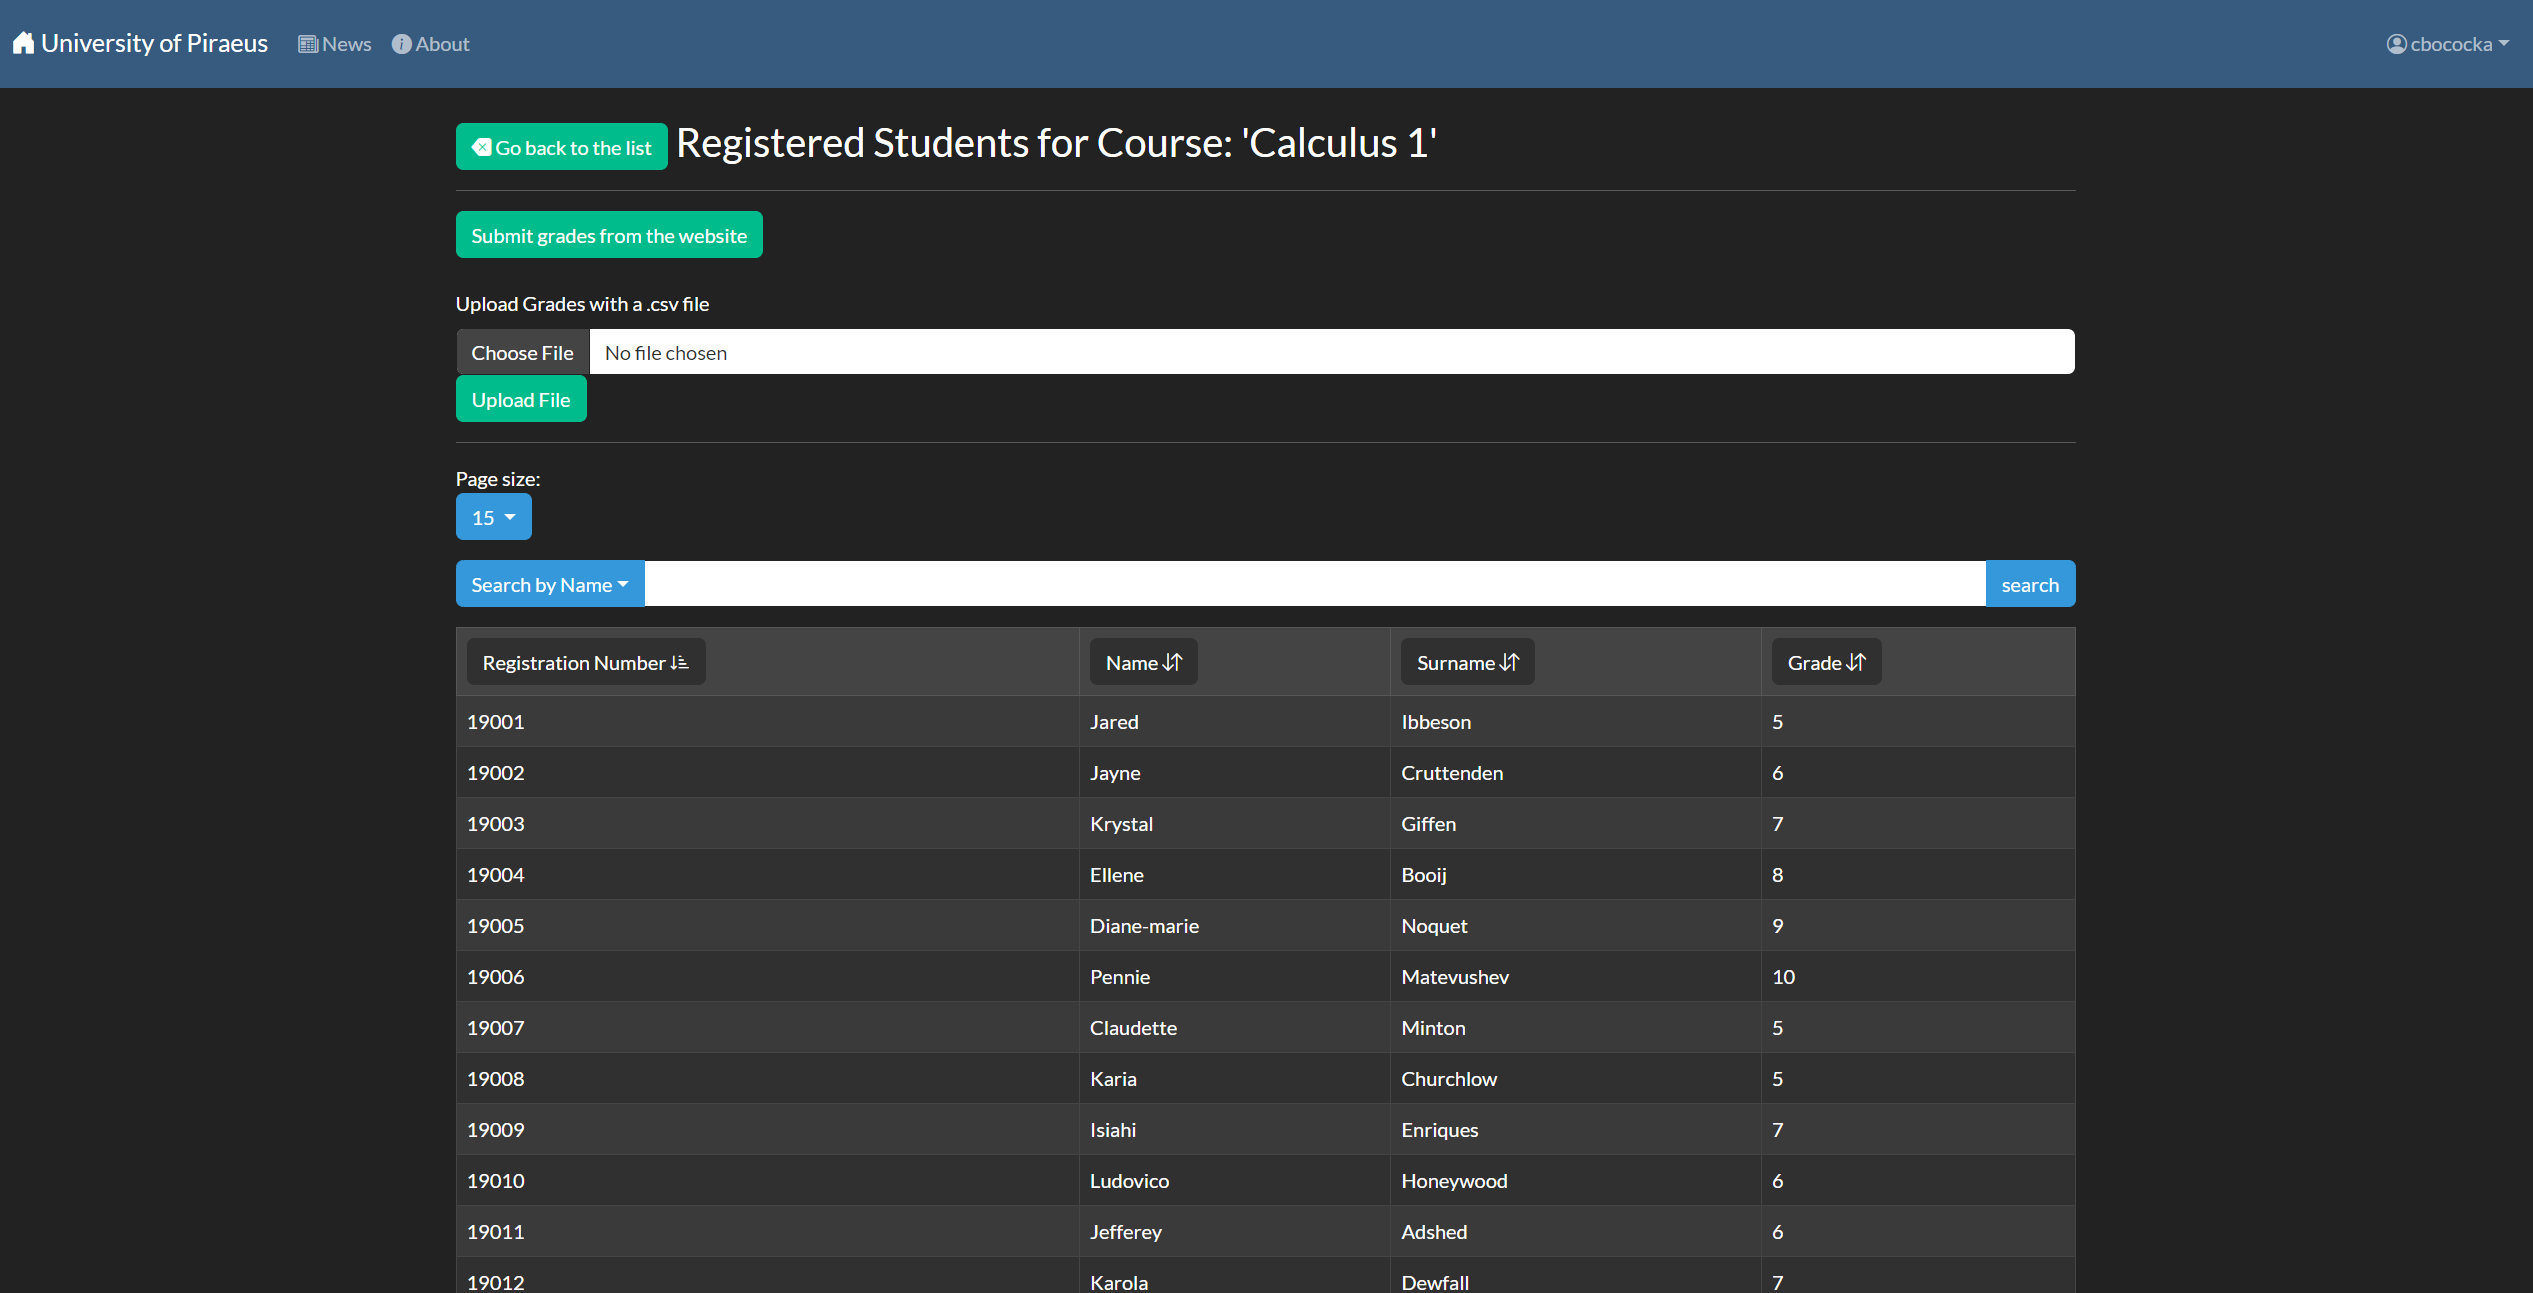
\includegraphics[width=0.85\textwidth]{mystudents.png}
		\caption{}
		\label{fig:emptyView}
	\end{figure}
	
	
	Μέσω αυτής της σελίδας ο καθηγητής μπορεί να εισάγει νέες βαθμολογίες με δύο τρόπους: 
	
	\begin{enumerate}
		\item μέσω της ιστοσελίδας πατώντας το κουμπί \textbf{'Submit grades from the website'}
		
		\item αναρώντας ενα .csv αρχείο μέσω των κουμπιών \textbf{'Choose File' και 'Upload File'}
	\end{enumerate}

	\subsection{Παράδειγμα ανάρτησης βαθμών μέσω της ιστοσελίδας}

	Κάνουμε κλικ στο κουμπί 'Go back to the list' και επιλέγουμε το μάθημα 'Data Structures' το οποίο περιέχει Φοιτητές που δεν έχουν βαθμούς. Ταξινομούμε τον πίνακα ως προς τη στήλη Grade.
	
	\begin{figure}[H]
		\centering
		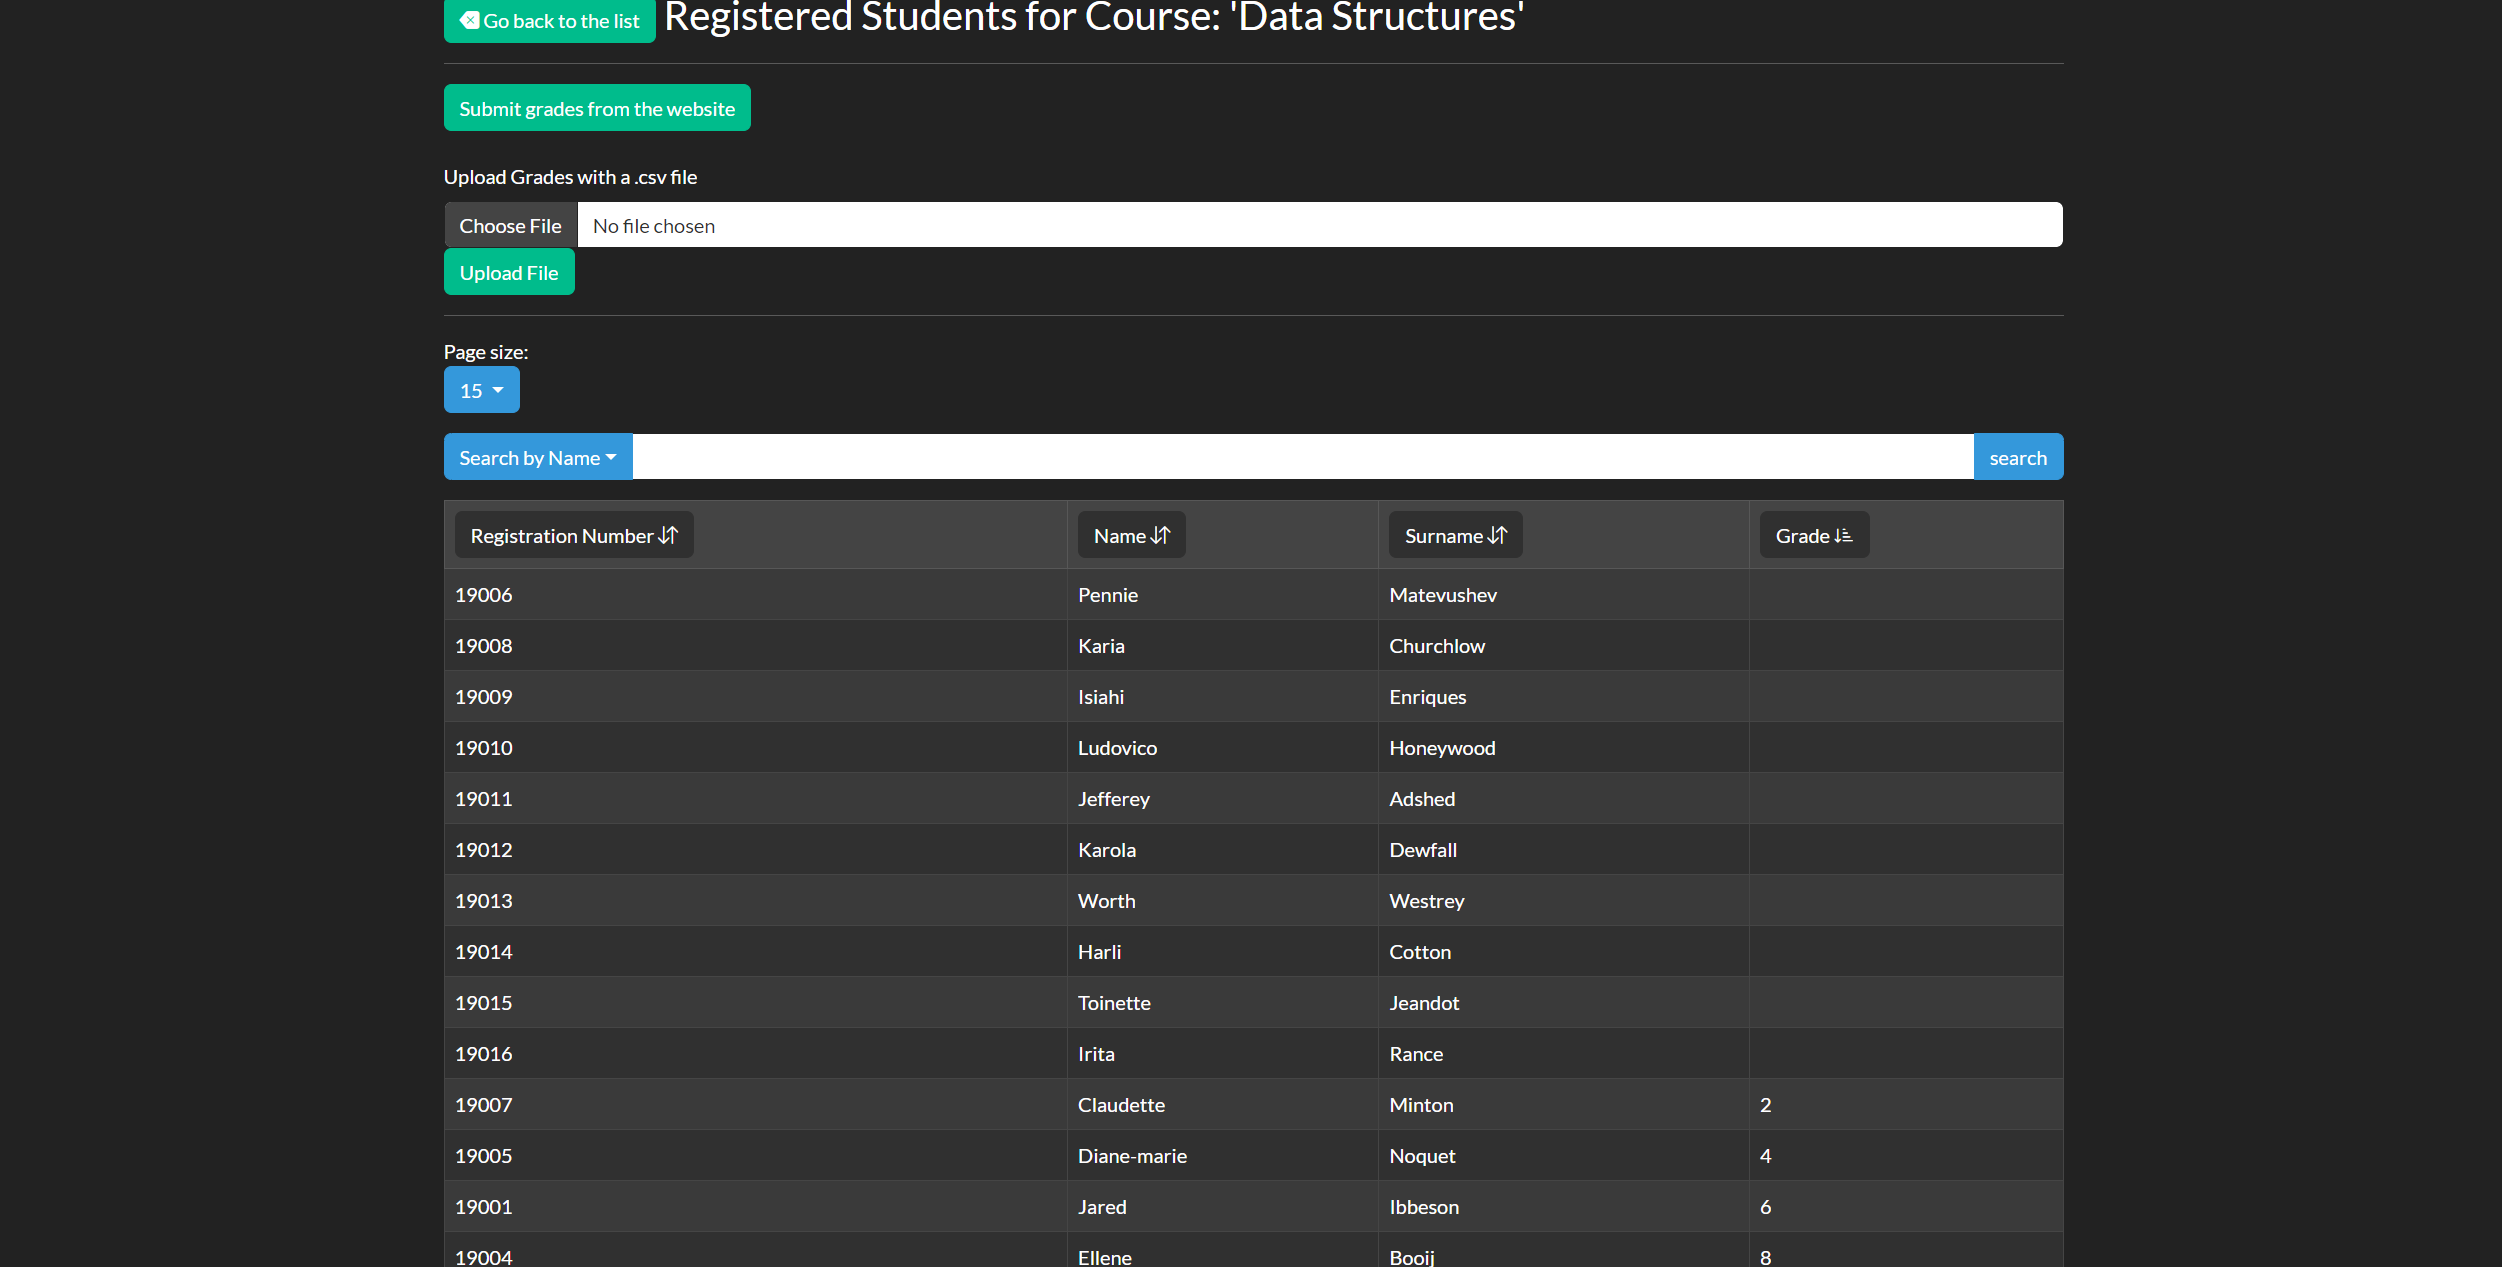
\includegraphics[width=0.85\textwidth]{datas.png}
		\caption{}
		\label{fig:emptyView}
	\end{figure}

	Επιλέγουμε \textbf{'Submit grades from the website'} και εμφανίζεται η παρακάτω ιστοσελίδα:
	
		\begin{figure}[H]
		\centering
		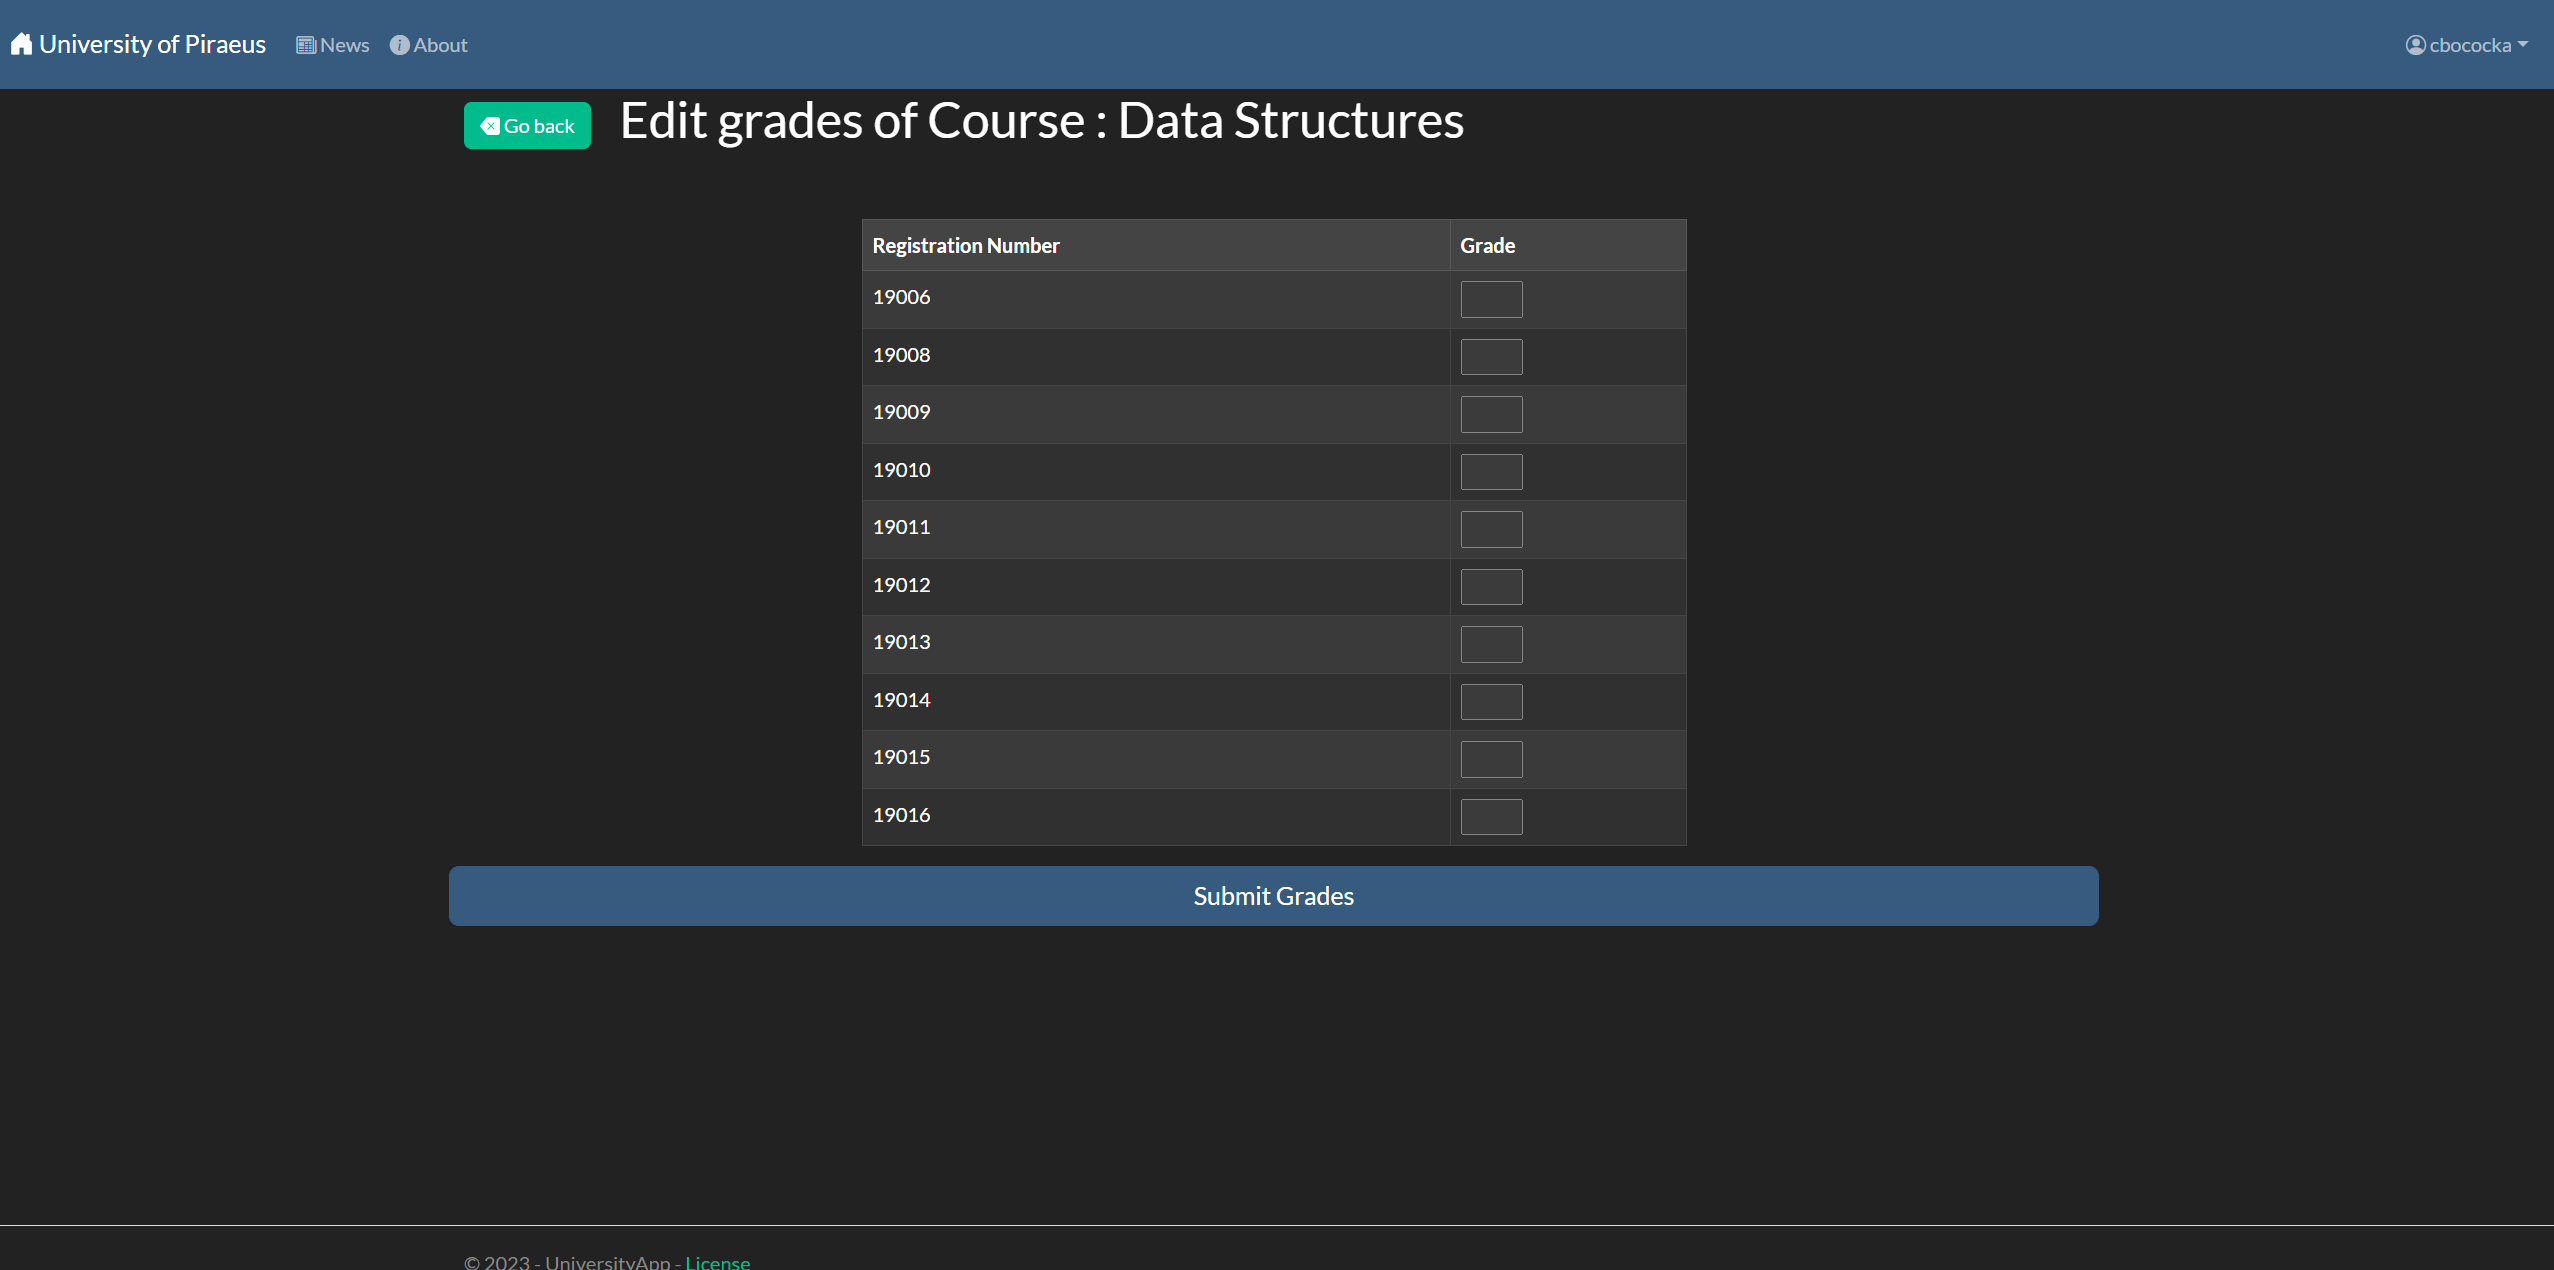
\includegraphics[width=0.85\textwidth]{edits23.png}
		\caption{}
		\label{fig:emptyView}
		\end{figure}
	
	Εδώ καλείται ο καθηγητής να συμπληρώσει τα πεδία που επιθυμεί με τον βαθμό του αντίστοιχου φοιτητή και να πατήσει \textbf{'Submit Grades'}. Αν ο καθηγητής συμπληρώσει μη έγκυρο βαθμό (μικρότερος του 0 ή μεγαλύτερος του 10) θα εμφανιστεί ένα απλό alert παράθυρο. Έστω συμπληρώνονται οι παρακάτω βαθμοί.
	
	\begin{figure}[H]
		\centering
		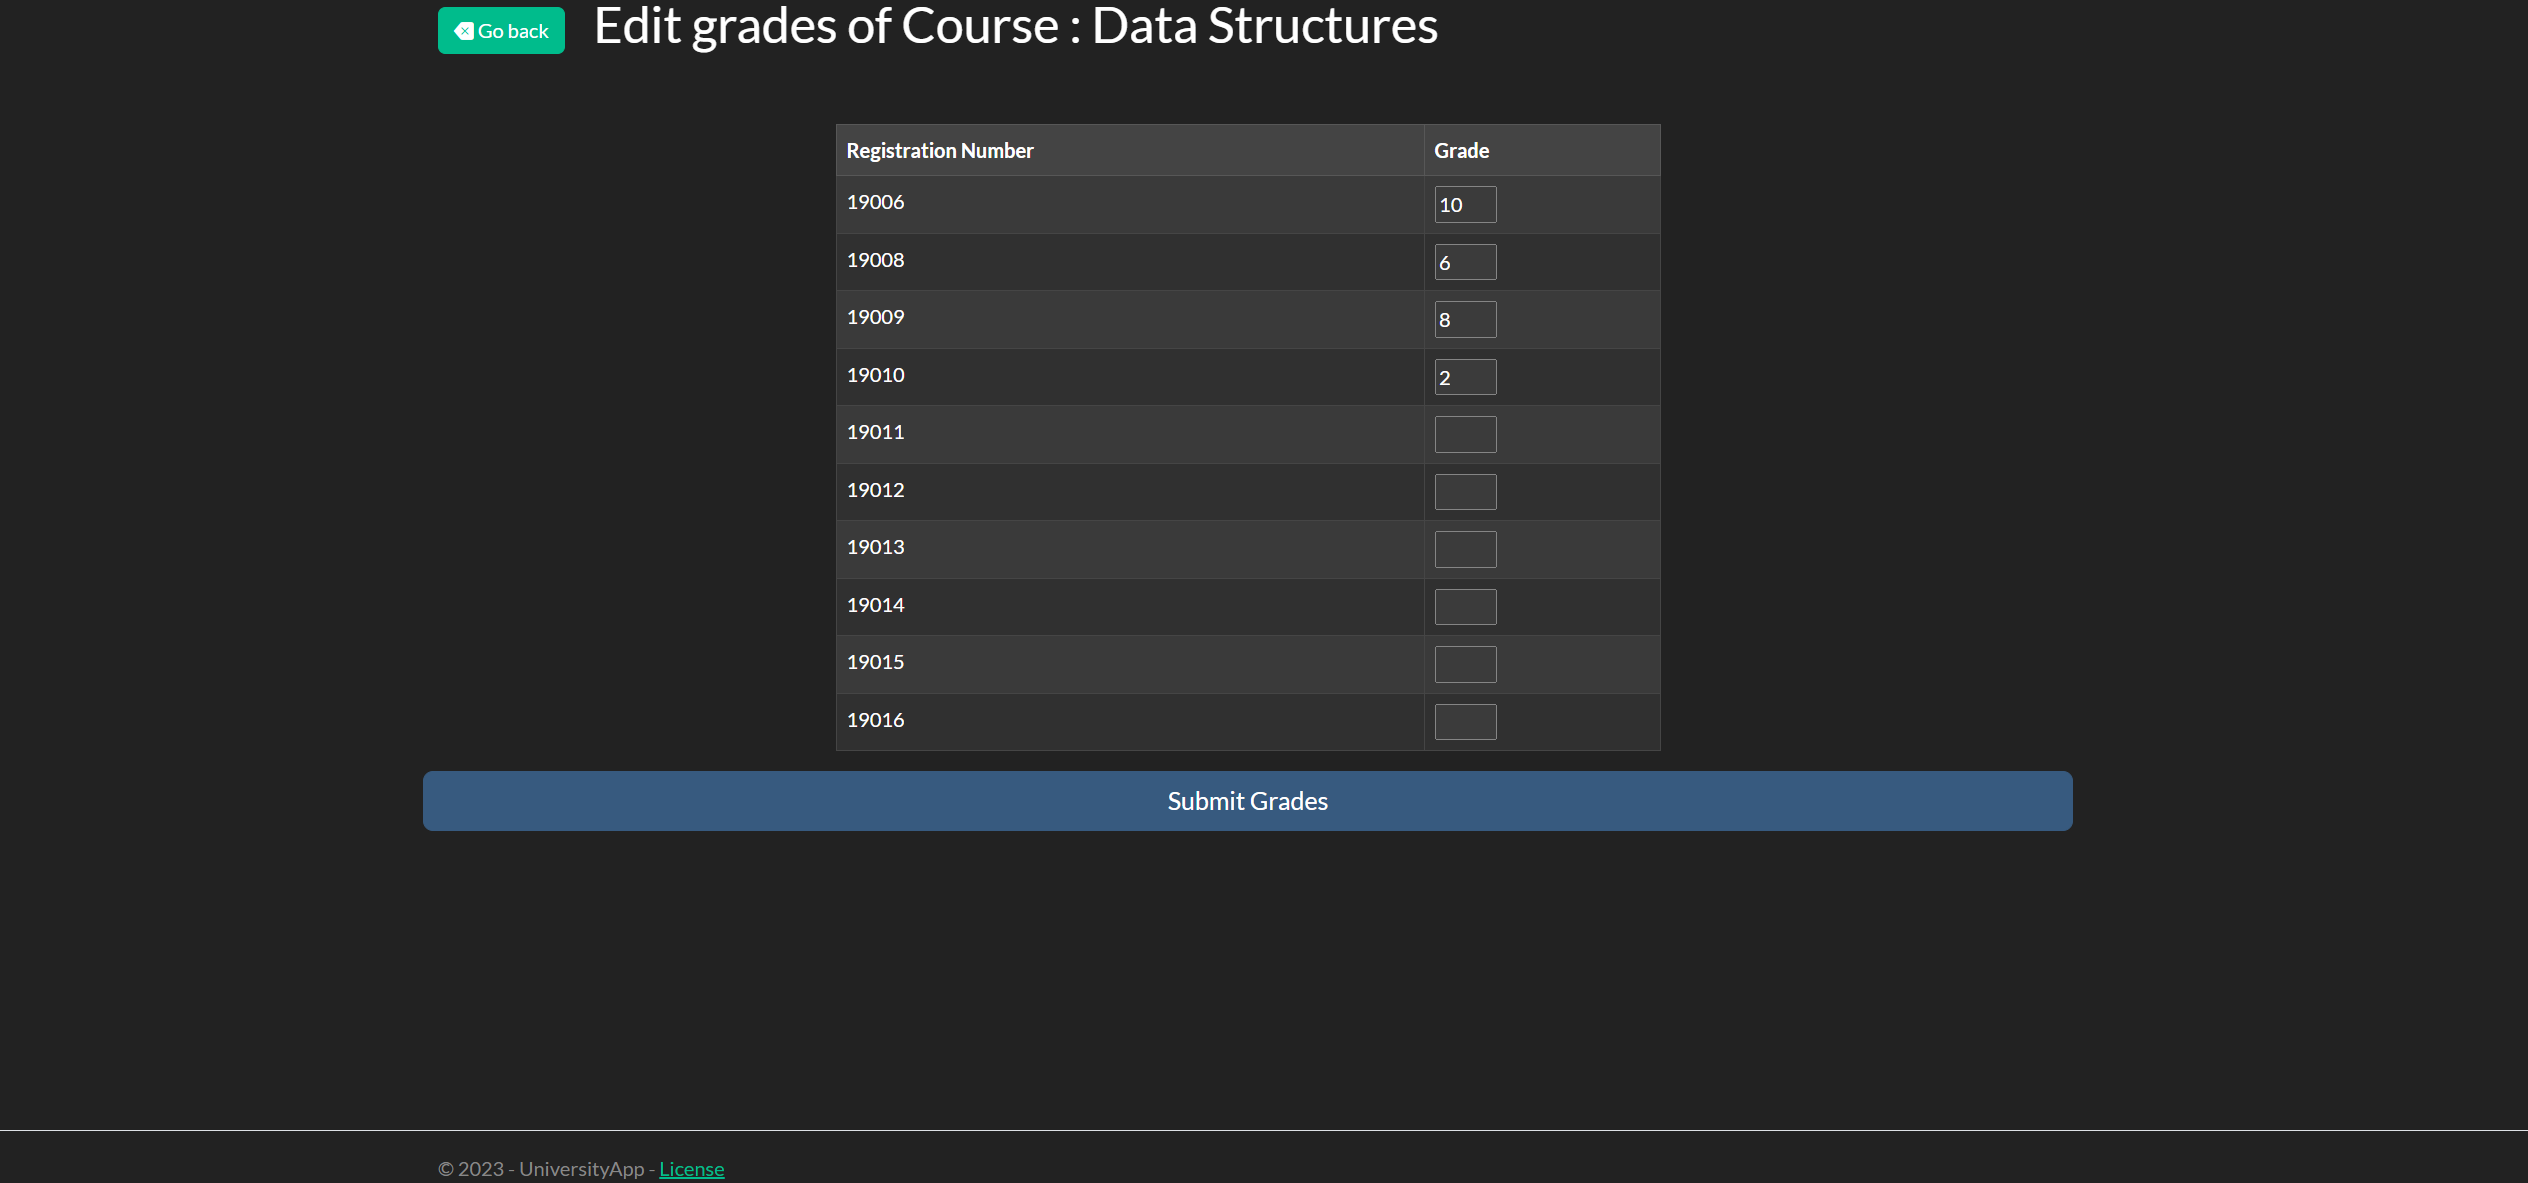
\includegraphics[width=0.85\textwidth]{edits234.png}
		\caption{}
		\label{fig:emptyView}
	\end{figure}

	Πατώντας \textbf{'Submit Grades'} επιστρέφουμε στην προηγούμενη σελίδα και όπως φαίνεται οι βαθμοί ενημερώθηκαν με επιτυχία.
	
	\begin{figure}[H]
		\centering
		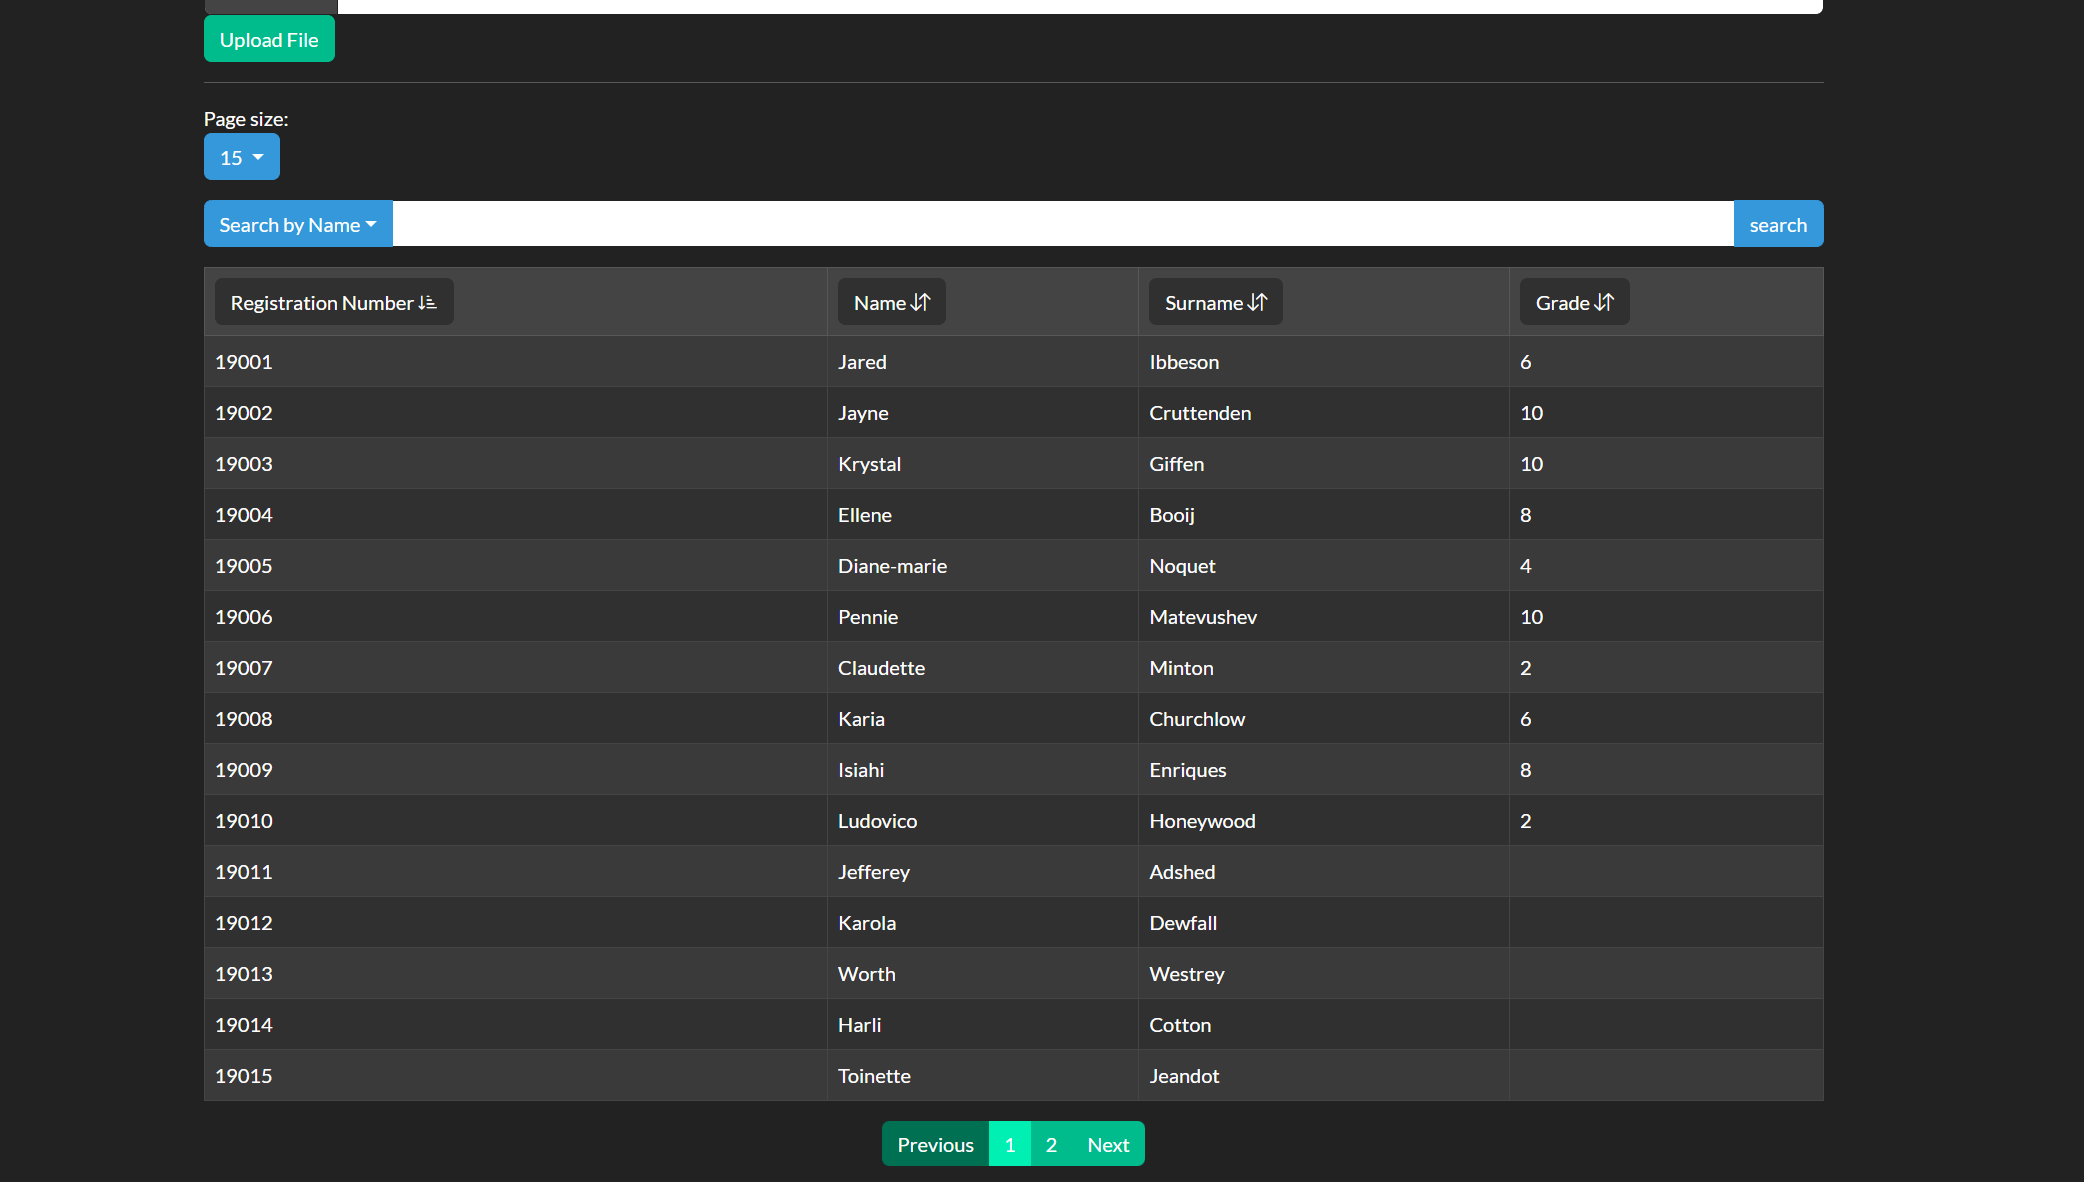
\includegraphics[width=0.85\textwidth]{newstudents.png}
		\caption{}
		\label{fig:emptyView}
	\end{figure}

	\subsection{Παράδειγμα ανάρτησης βαθμών μέσω της ιστοσελίδας}
	
	Μένοντας στην ίδια σελίδα, ταξινομούμε πάλι τον πίνακα με τη στήλη Grade ώστε να φανούν ποιοι φοιτητές δεν έχουν βαθμό.
	
	\begin{figure}[H]
	\centering
	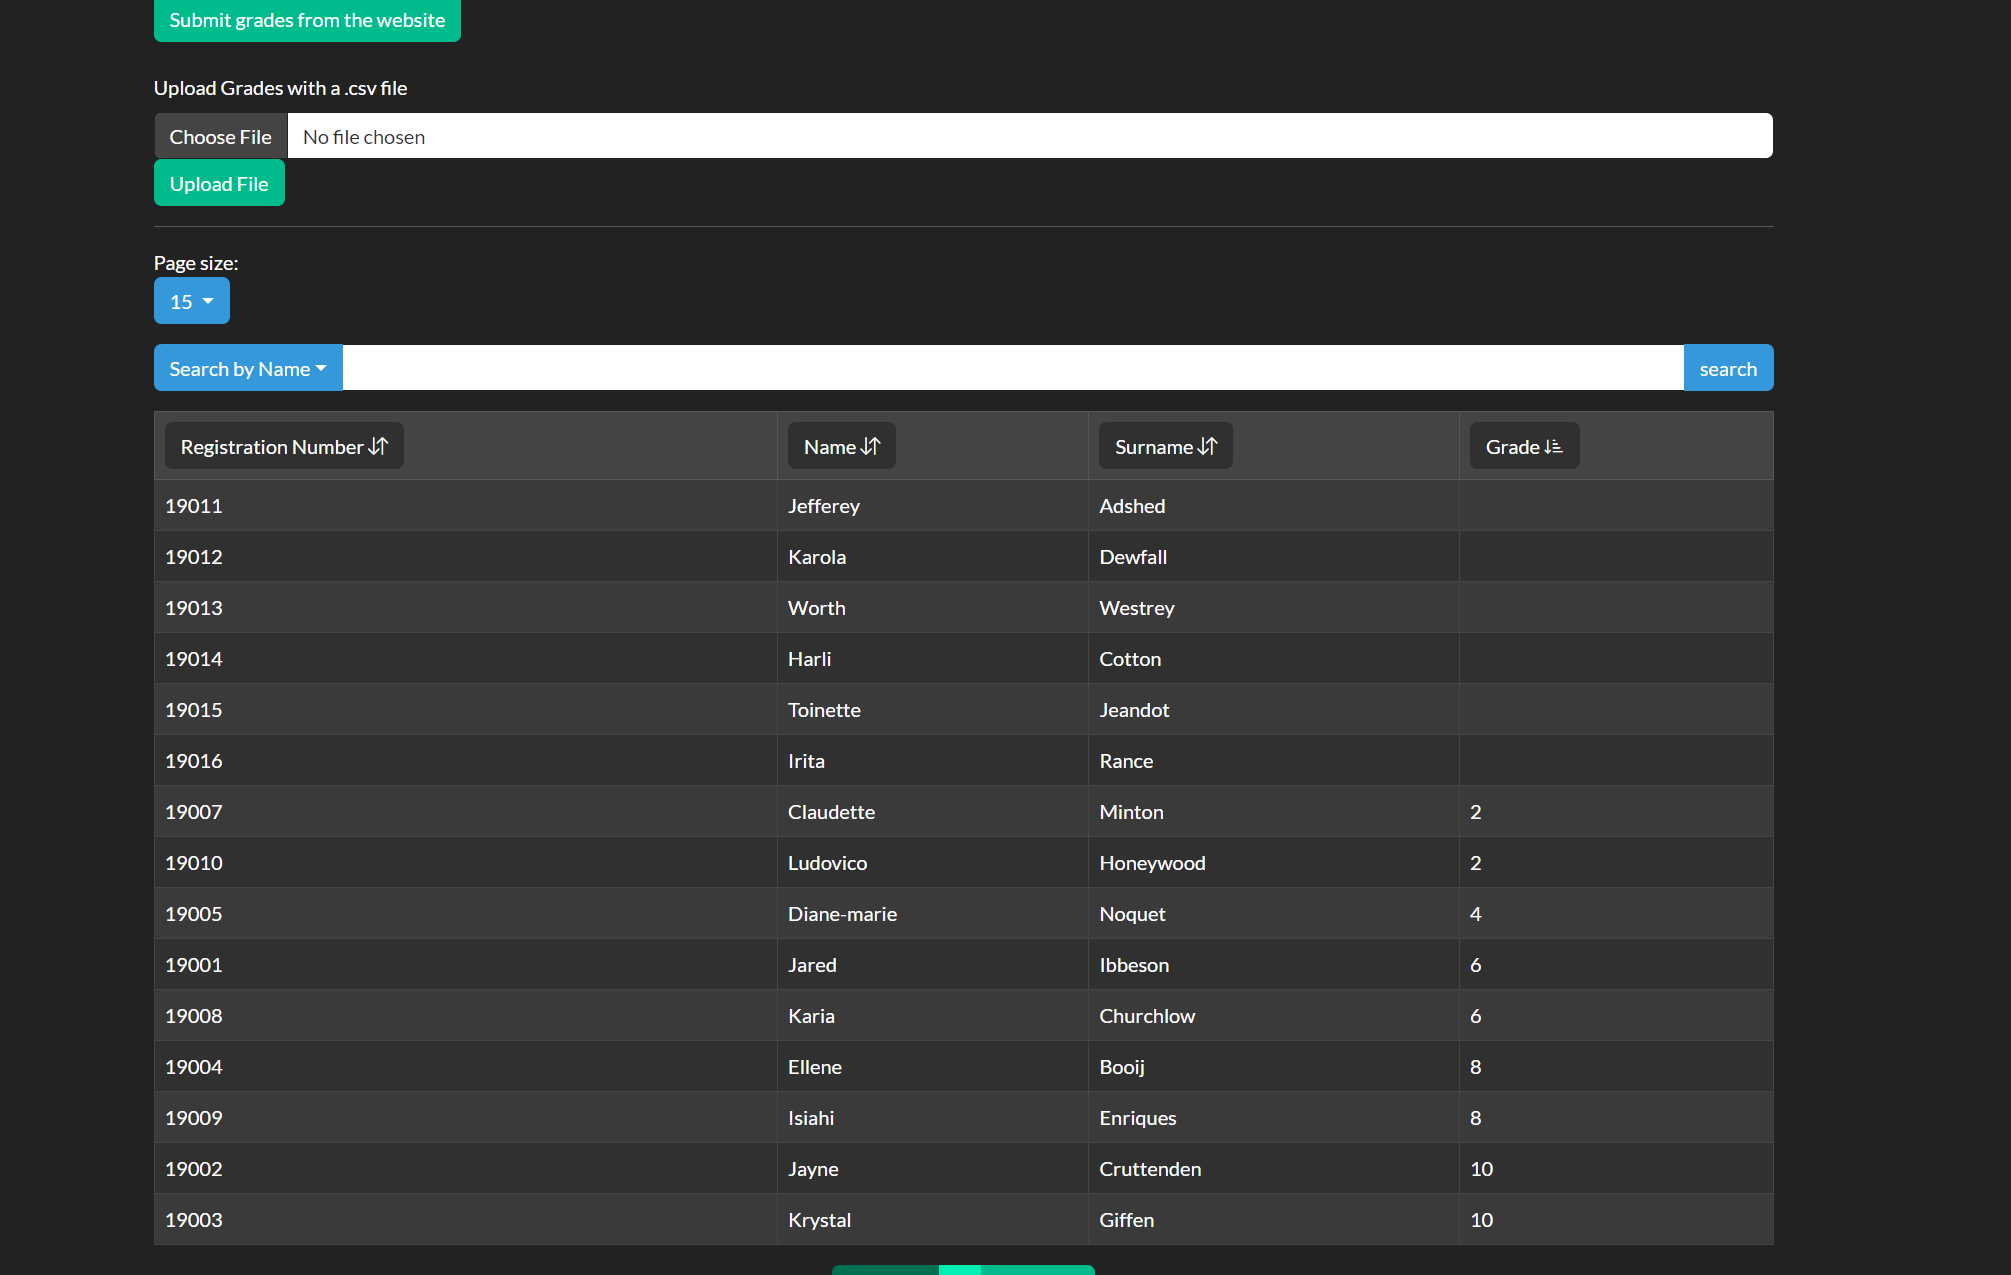
\includegraphics[width=0.85\textwidth]{mymy.png}
	\caption{}
	\label{fig:emptyView}
	\end{figure}

	Δημιουργούμε μέσω του Excel το παρακάτω .csv. Η πρώτη στήλη είναι το Registration Number και η δεύτερη ο βαθμός. Παρακάτω είναι ένα παράδειγμα ενός ορθού csv στο Excel
	
	\begin{figure}[H]
		\centering
		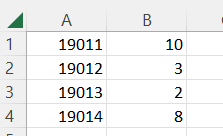
\includegraphics[width=0.22\textwidth]{correct.png}
		\caption{}
		\label{fig:emptyView}
	\end{figure}
	
	Αν το .csv περιέχει ΑΜ που δεν υπάρχουν στη βάση, δεν έχουν δηλώσει το μάθημα ή τα ΑΜ αντιστοιχούν σε φοιτητές που ήδη έχουν βαθμολογηθεί τα συγκεκριμένα ΑΜ θα αγνοηθούν. Επίσης αγνοούνται εγγραφές που έχουν μη έγκυρο βαθμό  (μικρότερο του 0 ή μεγαλύτερο του 10). Προσθέτουμε τις παρακάτω μη-έγκυρες εγγραφές.
	
	\begin{figure}[H]
		\centering
		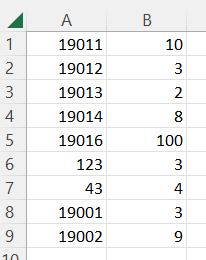
\includegraphics[width=0.25\textwidth]{wrong.png}
		\caption{}
		\label{fig:emptyView}
	\end{figure}
	
	Αναρτάμε το .csv στη σελίδα επιλέγοντας \textbf{'Choose File' και 'Upload File'}. Σε περίπτωση που υπάρχουν λάθη στο .csv (όπως εδώ) θα εμφανιστεί κατάλληλη σελίδα ώστε ο χρήστης να ενημερωθεί κατάλληλα (π.χ. έτσι μπορεί να ζητήσει ακριβώς ποιοι φοιτητές πρέπει να δηλώσουν το μάθημα ώστε να τους βαθμολογήσει).
	
	\begin{figure}[H]
		\centering
		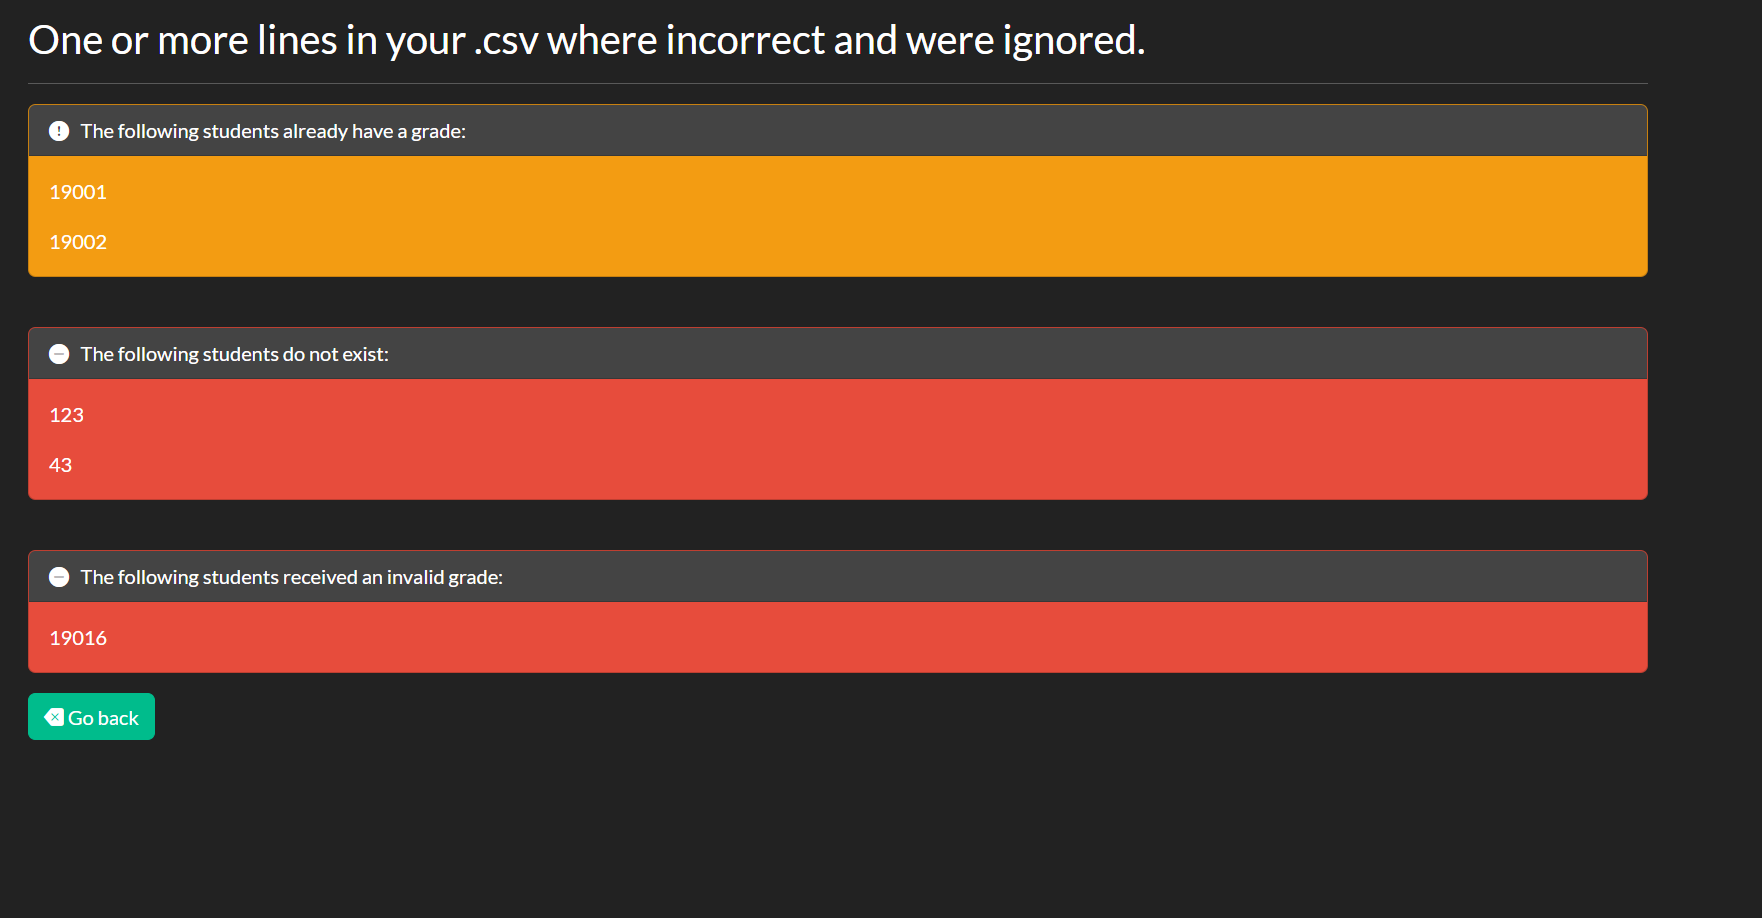
\includegraphics[width=0.85\textwidth]{reported.png}
		\caption{}
		\label{fig:emptyView}
	\end{figure}

	Επιλέγουμε Go back και βλέπουμε πως στη λίστα των φοιτητών πράγματι οι έγραφες που ήταν έγκυρες στο .csv πέρασαν με επιτυχία.

	\begin{figure}[H]
		\centering
		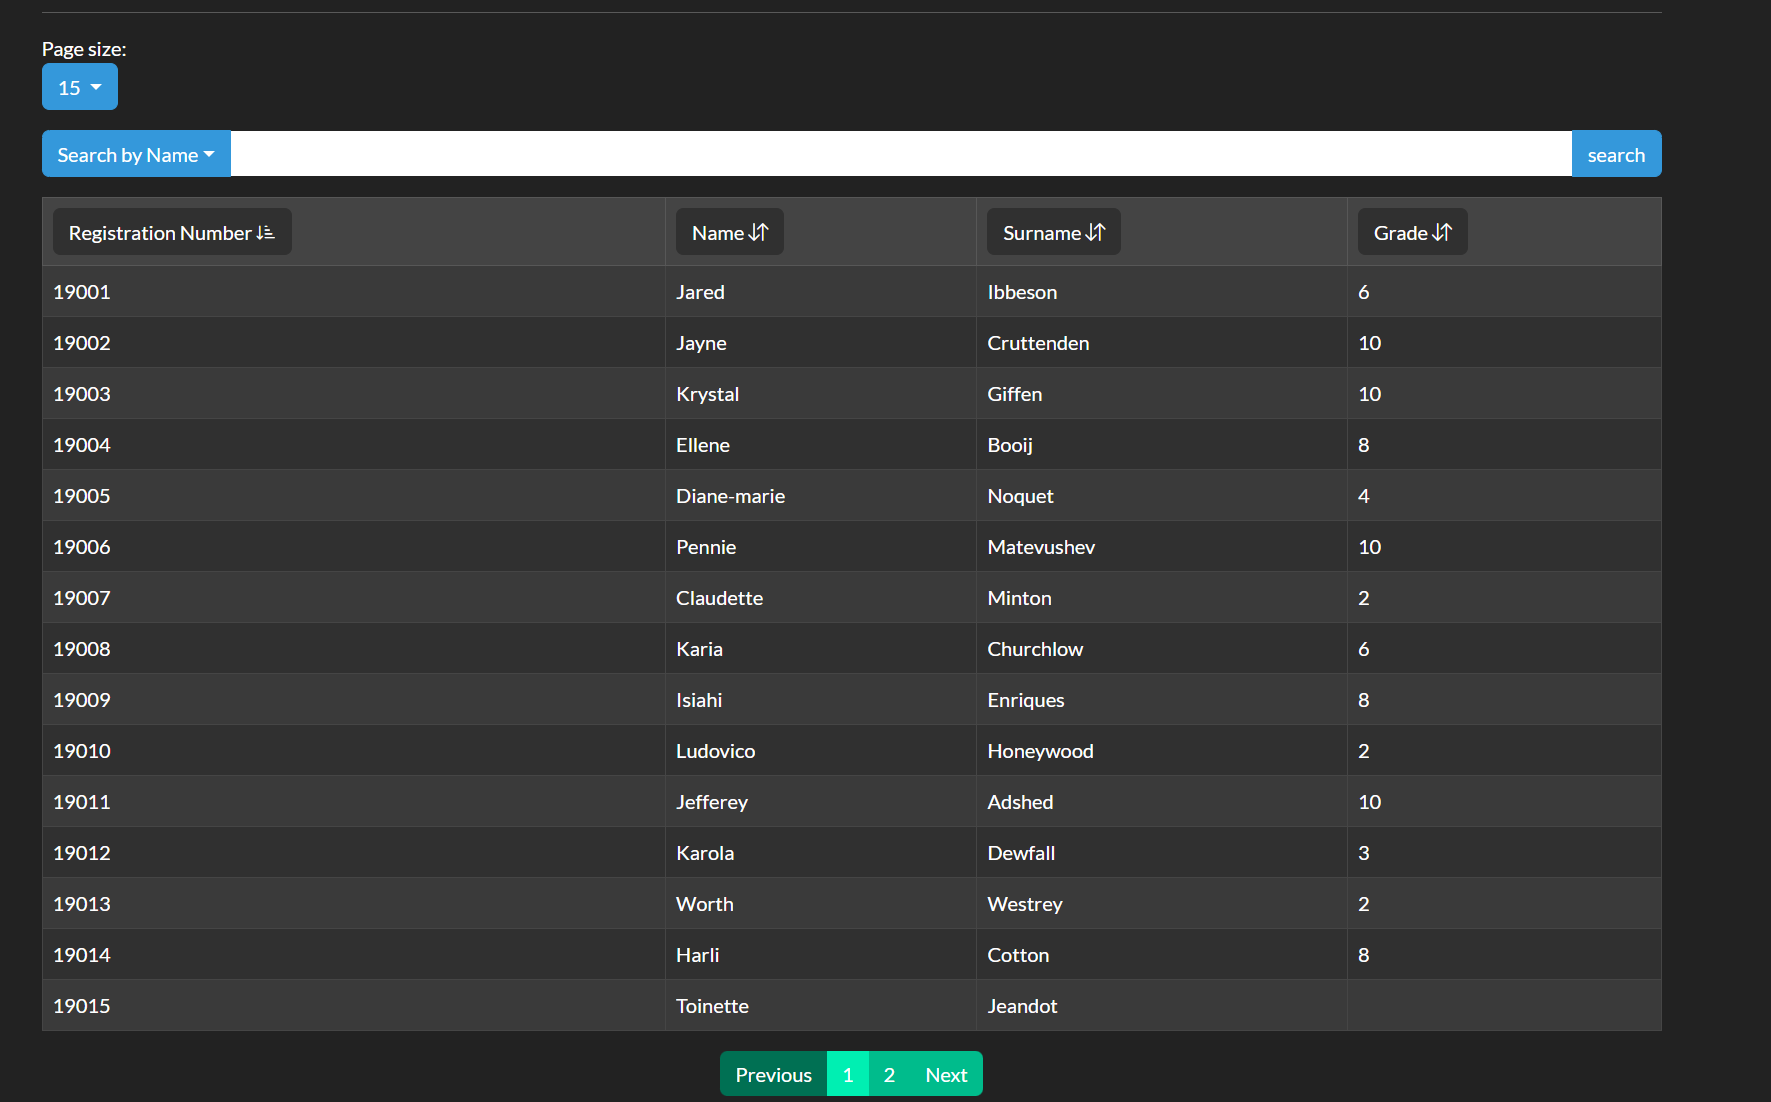
\includegraphics[width=0.85\textwidth]{cool.png}
		\caption{}
		\label{fig:emptyView}
	\end{figure}
	
	\newpage
	\subsection{Οδηγίες Γραμματείας}
	
		Όταν ο Γραμματέας δώσει τους σωστούς κωδικούς του θα μεταβεί στην παρακάτω σελίδα καλωσόρισης. Ενδεικτικά δίνονται τα παρακάτω credetials:
	
	\begin{itemize}
		\item Username : \textbf{aboyda0}
		\item Password : \textbf{Jgx8bp1zRC}
	\end{itemize}

	Σελίδα Φοιτητων
	
	εισαγωγη νεου φοιτητη
	Οπως αναφέρει η ενδειξη, θα δημιουργηθεί ένας λογαριασμός Φοιτητή με τα δοσμένα στοιχεία και Username ...
	λεπτομερειες ενος φοιτητη
	αναθεση μαθηματος σε φοιτητη
	Εμφανίζεται η λίστα μαθημάτων στην οποία ο γραμματέας τσεκαρει τα μαθήματα που θέλει να δηλωσει για τον συγκεκριμένο φοιτητή και πατάει submit
	
	Σελίδα Καθηγητών
	
	εισαγωγη νεου καθηγητη
	Οπως αναφέρει η ενδειξη, θα δημιουργηθεί ένας λογαριασμός Καθηγητή με τα δοσμένα στοιχεία και Username ...
	λεπτομερειες ενος καθηγητη
	αναθεση μαθηματος σε καθηγητη
	
	
	Σελίδα Μαθημάτων
	
	αναθεση ενός μαθηματος σε καθηγητη
	
	εισαγωγη νεου μαθηματος
	Μπορεί ο διαχειριστής να δηλώσει ποιος καθηγητής είναι υπεύθυνος για το μάθημα απο την δημιούργεια ή εκ των υστέρων
	λεπτομερειες ενος μαθήματος
	

		
		
	\end{document}
